%% Supplementary Information in the Springer Nature manuscript format.
\RequirePackage{xr-hyper}
\documentclass[pdflatex,referee]{../template/sn-jnl}
% A4 review layout: use the page instead of the class's small-format text block.
% Keep review line spacing; limit whitespace around figures and the title.
\geometry{reset,a4paper,left=22mm,right=24mm,top=20mm,bottom=22mm,
          bindingoffset=0mm,footskip=10mm}
\raggedbottom
\setlength{\floatsep}{10pt plus 2pt minus 2pt}
\setlength{\textfloatsep}{10pt plus 2pt minus 2pt}
\setlength{\intextsep}{10pt plus 2pt minus 2pt}
\renewcommand{\topfraction}{.95}
\renewcommand{\bottomfraction}{.90}
\renewcommand{\textfraction}{.05}
\renewcommand{\floatpagefraction}{.80}
\makeatletter
% Float-only pages start at the top instead of being vertically centred.
\setlength{\@fptop}{0pt}
\setlength{\@fpsep}{10pt plus 2pt minus 2pt}
\usepackage{etoolbox}
\patchcmd{\@maketitle}{\vskip21pt}{\vskip0pt}{}{}
% The class also inserts an empty opening box and an unused article-type row.
\patchcmd{\@maketitle}{\newpage\null}{\newpage}{}{\PackageError{synkit-layout}{Cannot remove title opening box}{Check the class title definition.}}
\patchcmd{\@maketitle}{{\hbox to \textwidth{{\Artcatfont\ArtType\hfill}\par}}}{}{}{\PackageError{synkit-layout}{Cannot remove unused article-type row}{Check the class title definition.}}
\patchcmd{\@maketitle}{\vskip20pt}{\vskip0pt}{}{\PackageError{synkit-layout}{Cannot remove title padding}{Check the class title definition.}}
\pretocmd{\Titlefont}{\def\baselinestretch{1}}{}{}
\patchcmd{\@maketitle}{\vskip36pt}{\vskip12pt}{}{}
\makeatother

% Capability marks for the software-scope table.  Defined here, in the shared
% preamble, because xr-hyper imports main.aux (and its caption) into the SI.
% Shape carries the meaning; the marks are distinguishable without colour.
\newcommand{\yes}{\ensuremath{\checkmark}}
\newcommand{\no}{\ensuremath{\times}}
\newcommand{\pmark}{\ensuremath{(\checkmark)}}
\newcommand{\rot}[1]{\rotatebox[origin=l]{90}{#1}}


% Uncomment if you want numbered sections in the SI:
% \setcounter{secnumdepth}{3}

% ----- encoding and typography -----
\usepackage[T1]{fontenc}
\usepackage{lmodern}
\usepackage{xcolor}
\usepackage{xspace}
\usepackage{microtype}

% ----- math / symbols -----
\usepackage{amsmath,amssymb,mathtools,amsthm}
\usepackage{mathrsfs}

% ----- figures, tables, floats -----
\usepackage{graphicx}
\usepackage{subcaption}
\usepackage{float}
\usepackage{booktabs}
\usepackage{tabularx}
\usepackage{longtable}
\usepackage{array}
\usepackage{multirow}
\usepackage{pdflscape}
\usepackage{adjustbox}
\usepackage{seqsplit}
\usepackage{enumitem}

% ----- chemistry / units -----
\usepackage{siunitx}
\usepackage[version=4]{mhchem}
\usepackage{chemfig}
\usepackage{tikz}
% The architecture figure is the TikZ source itself, not a compiled PDF.
\setchemfig{
  atom sep=2.4em,
  bond offset=2pt
}

% ----- code / listings -----
\usepackage{xcolor}
\usepackage{listings}
\lstset{
  basicstyle=\scriptsize\ttfamily\color{black},
  language=Python,
  keywordstyle=\color{blue},
  stringstyle=\color{olive},
  identifierstyle=\color{black},
  commentstyle=\color{gray},
  showstringspaces=false,
  frame=single,
  breaklines=true,
  breakatwhitespace=true,
  columns=fullflexible,
  keepspaces=true,
  upquote=true,
  captionpos=b,
  numbers=none,
  numberstyle=\tiny,
  xleftmargin=2.5em,
  xrightmargin=0.5em
}

% ----- bibliography -----
\usepackage[numbers,square]{natbib}
\bibliographystyle{../template/spbasic_u}

% ----- hyperlinks -----
\usepackage{hyperref}
\hypersetup{
  bookmarksdepth=2,
  colorlinks=true,
  linkcolor=blue,
  citecolor=blue,
  filecolor=blue,
  urlcolor=blue,
  anchorcolor=blue,
  pdfauthor={Thanh-An Pham and Tieu-Long Phan}
}

% (Cross-references into the main manuscript are declared after the project
% macros below, because xr-hyper expands the main manuscript's captions.)

% ----- theorem environments -----
\theoremstyle{plain}%
\newtheorem{theorem}{Theorem}
\newtheorem{proposition}[theorem]{Proposition}%
\theoremstyle{definition}%
\newtheorem{example}{Example}%
\newtheorem{remark}{Remark}%
\theoremstyle{remark}%
\newtheorem{definition}{Definition}

% ----- project macros -----
\newcommand{\synkit}{\texttt{SynKit}\xspace}
\newcommand{\synkitcrn}{\texttt{SynKit CRN}\xspace}
% BEGIN GENERATED: review-macros
\newcommand{\ReviewRandomMoietySeconds}{0.0514}
% END GENERATED: review-macros
\hyphenation{SynKit Bio-in-for-mat-ics Reactome Wiki-Pathways}

\newcommand{\pkg}[1]{\texttt{#1}\xspace}
\newcommand{\code}[1]{\texttt{#1}\xspace}
\newcommand{\class}[1]{\texttt{#1}\xspace}
\newcommand{\func}[1]{\texttt{#1()}\xspace}
\newcommand{\option}[1]{\texttt{#1}\xspace}
\newcommand{\smilescode}[1]{{\ttfamily\seqsplit{#1}}}
% Cross-references into the main manuscript, prefixed with `main:`.
\externaldocument[main:]{../main}

\newcommand{\figref}[1]{Fig.~\ref{#1}}
\newcommand{\tabref}[1]{Table~\ref{#1}}
\newcommand{\secref}[1]{Section~\ref{#1}}
\newcommand{\eqnref}[1]{Eq.~\eqref{#1}}
\newcommand{\doi}[1]{\href{https://doi.org/#1}{doi:#1}}
\newcommand{\pipcmd}[1]{\texttt{pip install #1}\xspace}
\newcommand{\pkgver}[2]{\pkg{#1}~(#2)\xspace}

% ----- siunitx config -----
\sisetup{
  detect-all,
  range-phrase = --,
  per-mode = symbol
}

% ----- caption style -----
\captionsetup{font=small,labelfont=bf}

% ----- supplementary numbering -----
\renewcommand{\thefigure}{S\arabic{figure}}
\renewcommand{\thetable}{S\arabic{table}}
\renewcommand{\thepage}{S\arabic{page}}
\AtBeginDocument{\renewcommand{\thelstlisting}{S\arabic{lstlisting}}}

\begin{document}

\title[Supplementary Information]{Supplementary Information\hb On The Conservation Laws and Pathway Realizability\hb of Biochemical Reaction Networks}

\author[1]{\fnm{Thanh-An} \sur{Pham}}\email{thanh-an.pham@uni-leipzig.de}
\author*[1,2]{\fnm{Tieu-Long} \sur{Phan}}\email{tieu@bioinf.uni-leipzig.de}

\affil[1]{\orgdiv{Bioinformatics Group, Department of Computer Science \& Interdisciplinary Center for Bioinformatics \& School for Embedded and Composite Artificial Intelligence (SECAI)}, \orgname{Leipzig University}, \orgaddress{\street{H{\"a}rtelstra{\ss}e 16--18}, \postcode{D-04107}, \city{Leipzig}, \country{Germany}}}
\affil[2]{\orgdiv{Department of Mathematics and Computer Science}, \orgname{University of Southern Denmark}, \orgaddress{\postcode{DK-5230}, \city{Odense M}, \country{Denmark}}}

\maketitle

\section{Software architecture and analysis interfaces}
\label{si:software}

Fig.~\ref{fig:synkit_architecture} shows the input adapters and analysis interfaces of the chemical reaction network (CRN) submodule of \synkit. The shared reaction-system representation preserves reactant and product multiplicities, so derived stoichiometric matrices, Petri nets, and hypergraphs refer to the same reaction records and species identifiers. These representations connect model import and rule expansion to structural analysis and finite-inventory pathway verification.

\begin{figure}[!htbp]
    \centering
    % ---------------------------------------------------------------------------
% arch.tex --- SynKit CRN at a glance: three routes in, one canonical object,
% views derived from it, and the analysis outputs that then apply.
%
% Source fragment: loaded directly by main.tex and SI/si.tex.
%
% Width.  The shared \scCanvas is pinned to the sn-jnl class default of 372 pt.
% paper_layout.tex replaces that text block with A4 at 22/24 mm margins, giving
% \textwidth = 466.63 pt = 16.40 cm, so a \scCanvas figure fills only 79.7% of
% the line.  This figure is therefore laid out on its own 16.40 cm canvas and
% included unscaled, so it fills the block at 1:1 and its type prints at the
% same physical size as every other figure's.
%
% Colour is semantic: green = structure, orange = the highlighted thing
% (the canonical object, the catalyst, the certificate), vermillion = a
% violation, and blue = a secondary/reference view.
%
% Text is deliberately sparse: the panels carry glyphs, the caption carries the
% qualifications.  Nothing here is a result.
% ---------------------------------------------------------------------------
% Resolve the shared style from the manuscript root or the SI directory.
\IfFileExists{synstyle.tex}{\input{synstyle}}{%
  \IfFileExists{Figure/synstyle.tex}{% ---------------------------------------------------------------------------
% synstyle.tex --- shared look for every TikZ figure of the SynKit CRN paper.
%
% Input it from a figure file:
%     \IfFileExists{synstyle.tex}{\input{synstyle}}{% ---------------------------------------------------------------------------
% synstyle.tex --- shared look for every TikZ figure of the SynKit CRN paper.
%
% Input it from a figure file:
%     \IfFileExists{synstyle.tex}{\input{synstyle}}{\input{Figure/synstyle}}
% so that the figure compiles both from Figure/ and from the paper root.
%
% The visual vocabulary follows ../../../../Style/style.tex: the
% colour-blind-safe Okabe--Ito accents, quiet neutral rules and wash, circular
% panel badges, and a compact technical type scale are shared by the companion
% papers.  Semantic aliases below keep the CRN meaning explicit.
%
% DESIGN CONTRACT -----------------------------------------------------------
% 1. Geometry.  Every figure is laid out on a canvas exactly \scW wide (the
%    sn-jnl text width, 372 pt) and is included unscaled, so one point of type
%    is the same physical size in all five figures.  Open each picture with
%    \scCanvas{<height in cm>} to pin the bounding box.
% 2. Colour is semantic, never decorative.  Four roles only:
%       scAccent (green)       structure, the normal/expected path
%       scMark   (orange)      catalyst, certificate, or highlight
%       scAlert  (vermillion)  failure, violation, or uncovered set
%       scRef    (blue)        secondary or reference series
%    A panel gets at most one accent.  Titles are always ink; panel identity
%    is also encoded by a letter inside a circular badge, not by colour alone.
% 3. Type scale.  Three sizes, no others, and nothing below 6 pt:
%       \scTitle (7 pt bold)  panel titles
%       \scBody  (6.5 pt)     labels, values, in-figure prose
%       \scSmall (6 pt)       units, footnotes, dense graph labels
% ---------------------------------------------------------------------------
% Load guard.  The paper inputs every figure source inline, so this file is
% reached once per figure; without the guard the second \newlength below
% would abort the run.
\ifdefined\SynKitStyleLoaded\endinput\fi
\newcommand{\SynKitStyleLoaded}{}

% Load in the document preamble. XeLaTeX/LuaLaTeX and an installed Arial
% family are required; fontspec reports an error instead of substituting.
\RequirePackage[no-math]{fontspec}
\newfontfamily\scArial{Arial}[NFSSFamily=scArial,Ligatures=TeX]
% Keep manuscript mathematics unchanged; select Arial letters and numerals
% only inside figures. TeX supplies specialist mathematical symbols.
\RequirePackage[subdued,italic]{mathastext}
\MTDeclareVersion{synarial}{TU}{scArial}{m}{n}
\SetMathAlphabet{\Mathsf}{synarial}{TU}{scArial}{m}{n}
\SetMathAlphabet{\Mathtt}{synarial}{TU}{scArial}{m}{n}

\usetikzlibrary{positioning,calc,fit,backgrounds,arrows.meta,shapes.geometric,
                shapes.misc,decorations.pathreplacing,patterns,math}

% --- canvas ---------------------------------------------------------------
% 372 pt text width minus the 1 pt standalone border on each side.
\newlength{\scW}\setlength{\scW}{13.0326cm}
\providecommand{\scWnum}{13.0326}
% \scCanvas{<height>} pins the picture to the full text width, y running down
% from 0, so every figure shares one coordinate convention.  It *sets* the
% bounding box rather than contributing to it, so the emitted page is exactly
% the text width and every figure is included at 1:1 -- otherwise a stray
% invisible extent (pgfplots reserves a little around an axis) rescales one
% figure relative to the others and the same \scSmall prints at two sizes.
% Anything drawn outside the canvas is therefore cropped: keep content inside,
% and check with
%     \providecommand{\scCanvas}[1]{\path[draw=red] (0,0) rectangle (\scWnum,-#1);}
\providecommand{\scCanvas}[1]{%
  \path[use as bounding box] (0,0) rectangle (\scWnum,-#1);}

% --- palette --------------------------------------------------------------
% Canonical companion-paper values (../../../../Style/style.tex).
\definecolor{npgOrange}{HTML}{E69F00}
\definecolor{npgSky}{HTML}{56B4E9}
\definecolor{npgGreen}{HTML}{009E73}
\definecolor{npgYellow}{HTML}{F0E442}
\definecolor{npgBlue}{HTML}{0072B2}
\definecolor{npgVermillion}{HTML}{E64B35}
\definecolor{npgPurple}{HTML}{CC79A7}
\definecolor{figInk}{HTML}{1A1A1A}
\definecolor{figMuted}{HTML}{666666}
\definecolor{figHair}{HTML}{D9D9D9}
\definecolor{figWash}{HTML}{F7F7F7}

\colorlet{scInk}{figInk}              % primary text
\colorlet{scInkM}{figMuted}           % secondary text
\colorlet{scPaper}{figWash}           % quiet cards and note strips
\colorlet{scSpF}{npgSky!12}           % species fill
\colorlet{scSpE}{npgBlue}             % species edge
\colorlet{scRxF}{npgOrange!12}        % reaction fill
\colorlet{scRxE}{npgOrange!88!black}  % reaction edge
\colorlet{scReac}{npgBlue!78!black}   % reactant edge
\colorlet{scProd}{npgGreen!82!black}  % product edge
\colorlet{scHiF}{npgOrange!13}        % highlight fill
\colorlet{scHiE}{npgOrange!82!black}  % highlight edge
% Stage / accent tints.  stDE remains available for the fifth plot series.
\colorlet{stAF}{npgGreen!9}\colorlet{stAE}{npgGreen}
\colorlet{stBF}{npgOrange!11}\colorlet{stBE}{npgOrange}
\colorlet{stCF}{npgBlue!9}\colorlet{stCE}{npgBlue}
\colorlet{stDF}{npgPurple!10}\colorlet{stDE}{npgPurple!85!black}
\colorlet{stEF}{npgVermillion!9}\colorlet{stEE}{npgVermillion}

% Semantic aliases.  Figures should speak in these, not in stAE/stBE/...
\colorlet{scAccent}{stAE}\colorlet{scAccentF}{stAF}   % structure / normal
\colorlet{scMark}{stBE}\colorlet{scMarkF}{stBF}       % highlight / certificate
\colorlet{scRef}{stCE}\colorlet{scRefF}{stCF}         % secondary series
\colorlet{scAlert}{stEE}\colorlet{scAlertF}{stEF}     % failure / violation
\colorlet{scRule}{figHair}                            % card and axis hairlines
\colorlet{scRuleL}{figHair!55}                        % grid, dividers

% --- text styles ----------------------------------------------------------
% Three sizes, fixed in points so they do not drift with the document class.
% Arial is shared by labels, headings, panel badges, and chemistry labels.
\providecommand{\scTitle}{\scArial\fontsize{7}{8.4}\selectfont\bfseries\color{scInk}}
\providecommand{\scBody}{\scArial\fontsize{6.5}{7.8}\selectfont\color{scInkM}}
\providecommand{\scSmall}{\scArial\fontsize{6}{7.2}\selectfont\color{scInkM}}
\providecommand{\scSub}[1]{{\scSmall\itshape #1}}
\providecommand{\scPanel}[1]{{\scTitle(#1)}}
% Numerals that carry a result: ink, not colour, so the eye reads the value.
\providecommand{\scNum}{\scArial\fontsize{10}{11}\selectfont\bfseries\color{scInk}}

% --- shared TikZ styles ---------------------------------------------------
\tikzset{
  % text never hyphenates inside a figure
  every node/.append style={execute at begin node={%
      \hyphenpenalty=10000 \exhyphenpenalty=10000 \hbadness=10000 }},
  syn/.style={font=\scArial,color=scInk,
              execute at begin picture={\MTversion*{synarial}},
              >={Stealth[round,length=2.4mm,width=1.9mm]}},
  % containers ------------------------------------------------------------
  % One card chrome for the whole paper: white, 3 pt radius, one hairline.
  panel/.style={rounded corners=2.5pt,fill=none,draw=scRule,line width=0.45pt},
  card/.style={rounded corners=2.2pt,fill=scPaper,draw=scRule,line width=0.45pt,
               inner sep=5pt,align=left,anchor=north west},
  % a quiet strip for a panel's closing fact
  note/.style={rounded corners=2.5pt,fill=scPaper,draw=scRuleL,line width=0.4pt,
               inner xsep=6pt,inner ysep=3.5pt,align=left,font=\scSmall},
  % small labelled value pill
  chip/.style={rounded corners=2pt,fill=scPaper,draw=scRule,line width=0.4pt,
               inner xsep=4pt,inner ysep=2pt,font=\scSmall},
  % Circular letter badge: the same accessible panel marker used in Style/*.
  hbullet/.style={circle,fill=scInk,text=white,draw=none,
                  font=\scArial\fontsize{6}{6}\selectfont\bfseries,
                  minimum size=4.2mm,inner sep=0pt},
  ctag/.style={font=\scTitle,anchor=north west,text=scInk},
  % CRN primitives --------------------------------------------------------
  species/.style={rounded rectangle,fill=scSpF,draw=scSpE,line width=0.45pt,
                  inner xsep=2.4pt,inner ysep=1.6pt,font=\scSmall,
                  text=scInk,minimum height=3.6mm},
  cofactor/.style={species,fill=scRefF,draw=scRef},
  catalyst/.style={species,fill=scHiF,draw=scHiE},
  rxn/.style={rectangle,fill=scRxF,draw=scRxE,line width=0.45pt,
              inner sep=1.2pt,font=\scSmall,text=scInk,
              minimum width=3.0mm,minimum height=3.0mm},
  place/.style={circle,fill=scSpF,draw=scSpE,line width=0.45pt,
                minimum size=4.0mm,inner sep=0pt},
  trans/.style={rectangle,fill=scRxE,draw=scRxE,minimum width=1.1mm,
                minimum height=3.6mm,inner sep=0pt},
  token/.style={circle,fill=scInk,minimum size=1.1mm,inner sep=0pt},
  % edges -----------------------------------------------------------------
  reac/.style={->,line width=0.5pt,draw=scReac,shorten >=0.8pt,shorten <=0.8pt},
  prod/.style={->,line width=0.5pt,draw=scProd,shorten >=0.8pt,shorten <=0.8pt},
  cat/.style={->,line width=0.5pt,draw=scHiE,shorten >=0.8pt,shorten <=0.8pt},
  flow/.style={-{Stealth[round,length=2.2mm,width=1.8mm]},line width=1.1pt,
               draw=scInkM!45},
  flab/.style={font=\scSmall,text=scInkM,inner sep=2pt},
  stoi/.style={font=\scSmall,text=scInkM,inner sep=0.8pt},
  % verdict marks: shape carries the meaning, colour only reinforces it
  vpass/.style={circle,fill=scAccentF,draw=scAccent,text=scAccent,
                font=\fontsize{6}{6}\selectfont\bfseries,
                minimum size=3.2mm,inner sep=0pt},
  vfail/.style={circle,fill=scAlertF,draw=scAlert,text=scAlert,
                font=\fontsize{6}{6}\selectfont\bfseries,
                minimum size=3.2mm,inner sep=0pt},
  callout/.style={font=\scSmall,text=scInkM,align=left},
}

% \scHead[<badge colour>]{<anchor coord>}{<letter>}{<title>}{<subtitle or empty>}
% One header treatment for every panel in the paper.
\providecommand{\scHead}[5][scInk]{%
  \node[hbullet,fill=#1,anchor=north west] (scbadge#3) at ($#2+(0,-0.015)$)
    {\MakeUppercase{#3}};
  \node[ctag,anchor=west] at ($(scbadge#3.east)+(0.14,0)$) {#4};
  \ifx\relax#5\relax\else
    \node[anchor=north west,font=\scSmall,text=scInkM]
      at ($#2+(0.56,-0.245)$) {#5};
  \fi}

% --- shared pgfplots look (only if the figure loaded pgfplots) ------------
\ifdefined\pgfplotsset
  \pgfplotsset{compat=1.18}
  \pgfplotsset{
    synaxis/.style={
      scale only axis,
      tick align=outside, tick pos=left,
      axis line style={draw=scInkM!55,line width=0.4pt},
      % One grid, on the value axis only.  No minor grid: at these sizes it
      % turns the plot frame into a grey wash.
      ymajorgrids=true, xmajorgrids=false,
      major grid style={draw=scRuleL,line width=0.3pt},
      major tick length=1.6pt,
      label style={font=\scBody,color=scInk},
      tick label style={font=\scSmall,color=scInkM},
      legend style={font=\scSmall,draw=none,fill=none,inner sep=1pt,
                    row sep=0.4pt,legend columns=1},
      legend cell align=left,
      every axis plot/.append style={line width=0.7pt,mark size=1.2pt},
    },
  }
\fi
}
% so that the figure compiles both from Figure/ and from the paper root.
%
% The visual vocabulary follows ../../../../Style/style.tex: the
% colour-blind-safe Okabe--Ito accents, quiet neutral rules and wash, circular
% panel badges, and a compact technical type scale are shared by the companion
% papers.  Semantic aliases below keep the CRN meaning explicit.
%
% DESIGN CONTRACT -----------------------------------------------------------
% 1. Geometry.  Every figure is laid out on a canvas exactly \scW wide (the
%    sn-jnl text width, 372 pt) and is included unscaled, so one point of type
%    is the same physical size in all five figures.  Open each picture with
%    \scCanvas{<height in cm>} to pin the bounding box.
% 2. Colour is semantic, never decorative.  Four roles only:
%       scAccent (green)       structure, the normal/expected path
%       scMark   (orange)      catalyst, certificate, or highlight
%       scAlert  (vermillion)  failure, violation, or uncovered set
%       scRef    (blue)        secondary or reference series
%    A panel gets at most one accent.  Titles are always ink; panel identity
%    is also encoded by a letter inside a circular badge, not by colour alone.
% 3. Type scale.  Three sizes, no others, and nothing below 6 pt:
%       \scTitle (7 pt bold)  panel titles
%       \scBody  (6.5 pt)     labels, values, in-figure prose
%       \scSmall (6 pt)       units, footnotes, dense graph labels
% ---------------------------------------------------------------------------
% Load guard.  The paper inputs every figure source inline, so this file is
% reached once per figure; without the guard the second \newlength below
% would abort the run.
\ifdefined\SynKitStyleLoaded\endinput\fi
\newcommand{\SynKitStyleLoaded}{}

% Load in the document preamble. XeLaTeX/LuaLaTeX and an installed Arial
% family are required; fontspec reports an error instead of substituting.
\RequirePackage[no-math]{fontspec}
\newfontfamily\scArial{Arial}[NFSSFamily=scArial,Ligatures=TeX]
% Keep manuscript mathematics unchanged; select Arial letters and numerals
% only inside figures. TeX supplies specialist mathematical symbols.
\RequirePackage[subdued,italic]{mathastext}
\MTDeclareVersion{synarial}{TU}{scArial}{m}{n}
\SetMathAlphabet{\Mathsf}{synarial}{TU}{scArial}{m}{n}
\SetMathAlphabet{\Mathtt}{synarial}{TU}{scArial}{m}{n}

\usetikzlibrary{positioning,calc,fit,backgrounds,arrows.meta,shapes.geometric,
                shapes.misc,decorations.pathreplacing,patterns,math}

% --- canvas ---------------------------------------------------------------
% 372 pt text width minus the 1 pt standalone border on each side.
\newlength{\scW}\setlength{\scW}{13.0326cm}
\providecommand{\scWnum}{13.0326}
% \scCanvas{<height>} pins the picture to the full text width, y running down
% from 0, so every figure shares one coordinate convention.  It *sets* the
% bounding box rather than contributing to it, so the emitted page is exactly
% the text width and every figure is included at 1:1 -- otherwise a stray
% invisible extent (pgfplots reserves a little around an axis) rescales one
% figure relative to the others and the same \scSmall prints at two sizes.
% Anything drawn outside the canvas is therefore cropped: keep content inside,
% and check with
%     \providecommand{\scCanvas}[1]{\path[draw=red] (0,0) rectangle (\scWnum,-#1);}
\providecommand{\scCanvas}[1]{%
  \path[use as bounding box] (0,0) rectangle (\scWnum,-#1);}

% --- palette --------------------------------------------------------------
% Canonical companion-paper values (../../../../Style/style.tex).
\definecolor{npgOrange}{HTML}{E69F00}
\definecolor{npgSky}{HTML}{56B4E9}
\definecolor{npgGreen}{HTML}{009E73}
\definecolor{npgYellow}{HTML}{F0E442}
\definecolor{npgBlue}{HTML}{0072B2}
\definecolor{npgVermillion}{HTML}{E64B35}
\definecolor{npgPurple}{HTML}{CC79A7}
\definecolor{figInk}{HTML}{1A1A1A}
\definecolor{figMuted}{HTML}{666666}
\definecolor{figHair}{HTML}{D9D9D9}
\definecolor{figWash}{HTML}{F7F7F7}

\colorlet{scInk}{figInk}              % primary text
\colorlet{scInkM}{figMuted}           % secondary text
\colorlet{scPaper}{figWash}           % quiet cards and note strips
\colorlet{scSpF}{npgSky!12}           % species fill
\colorlet{scSpE}{npgBlue}             % species edge
\colorlet{scRxF}{npgOrange!12}        % reaction fill
\colorlet{scRxE}{npgOrange!88!black}  % reaction edge
\colorlet{scReac}{npgBlue!78!black}   % reactant edge
\colorlet{scProd}{npgGreen!82!black}  % product edge
\colorlet{scHiF}{npgOrange!13}        % highlight fill
\colorlet{scHiE}{npgOrange!82!black}  % highlight edge
% Stage / accent tints.  stDE remains available for the fifth plot series.
\colorlet{stAF}{npgGreen!9}\colorlet{stAE}{npgGreen}
\colorlet{stBF}{npgOrange!11}\colorlet{stBE}{npgOrange}
\colorlet{stCF}{npgBlue!9}\colorlet{stCE}{npgBlue}
\colorlet{stDF}{npgPurple!10}\colorlet{stDE}{npgPurple!85!black}
\colorlet{stEF}{npgVermillion!9}\colorlet{stEE}{npgVermillion}

% Semantic aliases.  Figures should speak in these, not in stAE/stBE/...
\colorlet{scAccent}{stAE}\colorlet{scAccentF}{stAF}   % structure / normal
\colorlet{scMark}{stBE}\colorlet{scMarkF}{stBF}       % highlight / certificate
\colorlet{scRef}{stCE}\colorlet{scRefF}{stCF}         % secondary series
\colorlet{scAlert}{stEE}\colorlet{scAlertF}{stEF}     % failure / violation
\colorlet{scRule}{figHair}                            % card and axis hairlines
\colorlet{scRuleL}{figHair!55}                        % grid, dividers

% --- text styles ----------------------------------------------------------
% Three sizes, fixed in points so they do not drift with the document class.
% Arial is shared by labels, headings, panel badges, and chemistry labels.
\providecommand{\scTitle}{\scArial\fontsize{7}{8.4}\selectfont\bfseries\color{scInk}}
\providecommand{\scBody}{\scArial\fontsize{6.5}{7.8}\selectfont\color{scInkM}}
\providecommand{\scSmall}{\scArial\fontsize{6}{7.2}\selectfont\color{scInkM}}
\providecommand{\scSub}[1]{{\scSmall\itshape #1}}
\providecommand{\scPanel}[1]{{\scTitle(#1)}}
% Numerals that carry a result: ink, not colour, so the eye reads the value.
\providecommand{\scNum}{\scArial\fontsize{10}{11}\selectfont\bfseries\color{scInk}}

% --- shared TikZ styles ---------------------------------------------------
\tikzset{
  % text never hyphenates inside a figure
  every node/.append style={execute at begin node={%
      \hyphenpenalty=10000 \exhyphenpenalty=10000 \hbadness=10000 }},
  syn/.style={font=\scArial,color=scInk,
              execute at begin picture={\MTversion*{synarial}},
              >={Stealth[round,length=2.4mm,width=1.9mm]}},
  % containers ------------------------------------------------------------
  % One card chrome for the whole paper: white, 3 pt radius, one hairline.
  panel/.style={rounded corners=2.5pt,fill=none,draw=scRule,line width=0.45pt},
  card/.style={rounded corners=2.2pt,fill=scPaper,draw=scRule,line width=0.45pt,
               inner sep=5pt,align=left,anchor=north west},
  % a quiet strip for a panel's closing fact
  note/.style={rounded corners=2.5pt,fill=scPaper,draw=scRuleL,line width=0.4pt,
               inner xsep=6pt,inner ysep=3.5pt,align=left,font=\scSmall},
  % small labelled value pill
  chip/.style={rounded corners=2pt,fill=scPaper,draw=scRule,line width=0.4pt,
               inner xsep=4pt,inner ysep=2pt,font=\scSmall},
  % Circular letter badge: the same accessible panel marker used in Style/*.
  hbullet/.style={circle,fill=scInk,text=white,draw=none,
                  font=\scArial\fontsize{6}{6}\selectfont\bfseries,
                  minimum size=4.2mm,inner sep=0pt},
  ctag/.style={font=\scTitle,anchor=north west,text=scInk},
  % CRN primitives --------------------------------------------------------
  species/.style={rounded rectangle,fill=scSpF,draw=scSpE,line width=0.45pt,
                  inner xsep=2.4pt,inner ysep=1.6pt,font=\scSmall,
                  text=scInk,minimum height=3.6mm},
  cofactor/.style={species,fill=scRefF,draw=scRef},
  catalyst/.style={species,fill=scHiF,draw=scHiE},
  rxn/.style={rectangle,fill=scRxF,draw=scRxE,line width=0.45pt,
              inner sep=1.2pt,font=\scSmall,text=scInk,
              minimum width=3.0mm,minimum height=3.0mm},
  place/.style={circle,fill=scSpF,draw=scSpE,line width=0.45pt,
                minimum size=4.0mm,inner sep=0pt},
  trans/.style={rectangle,fill=scRxE,draw=scRxE,minimum width=1.1mm,
                minimum height=3.6mm,inner sep=0pt},
  token/.style={circle,fill=scInk,minimum size=1.1mm,inner sep=0pt},
  % edges -----------------------------------------------------------------
  reac/.style={->,line width=0.5pt,draw=scReac,shorten >=0.8pt,shorten <=0.8pt},
  prod/.style={->,line width=0.5pt,draw=scProd,shorten >=0.8pt,shorten <=0.8pt},
  cat/.style={->,line width=0.5pt,draw=scHiE,shorten >=0.8pt,shorten <=0.8pt},
  flow/.style={-{Stealth[round,length=2.2mm,width=1.8mm]},line width=1.1pt,
               draw=scInkM!45},
  flab/.style={font=\scSmall,text=scInkM,inner sep=2pt},
  stoi/.style={font=\scSmall,text=scInkM,inner sep=0.8pt},
  % verdict marks: shape carries the meaning, colour only reinforces it
  vpass/.style={circle,fill=scAccentF,draw=scAccent,text=scAccent,
                font=\fontsize{6}{6}\selectfont\bfseries,
                minimum size=3.2mm,inner sep=0pt},
  vfail/.style={circle,fill=scAlertF,draw=scAlert,text=scAlert,
                font=\fontsize{6}{6}\selectfont\bfseries,
                minimum size=3.2mm,inner sep=0pt},
  callout/.style={font=\scSmall,text=scInkM,align=left},
}

% \scHead[<badge colour>]{<anchor coord>}{<letter>}{<title>}{<subtitle or empty>}
% One header treatment for every panel in the paper.
\providecommand{\scHead}[5][scInk]{%
  \node[hbullet,fill=#1,anchor=north west] (scbadge#3) at ($#2+(0,-0.015)$)
    {\MakeUppercase{#3}};
  \node[ctag,anchor=west] at ($(scbadge#3.east)+(0.14,0)$) {#4};
  \ifx\relax#5\relax\else
    \node[anchor=north west,font=\scSmall,text=scInkM]
      at ($#2+(0.56,-0.245)$) {#5};
  \fi}

% --- shared pgfplots look (only if the figure loaded pgfplots) ------------
\ifdefined\pgfplotsset
  \pgfplotsset{compat=1.18}
  \pgfplotsset{
    synaxis/.style={
      scale only axis,
      tick align=outside, tick pos=left,
      axis line style={draw=scInkM!55,line width=0.4pt},
      % One grid, on the value axis only.  No minor grid: at these sizes it
      % turns the plot frame into a grey wash.
      ymajorgrids=true, xmajorgrids=false,
      major grid style={draw=scRuleL,line width=0.3pt},
      major tick length=1.6pt,
      label style={font=\scBody,color=scInk},
      tick label style={font=\scSmall,color=scInkM},
      legend style={font=\scSmall,draw=none,fill=none,inner sep=1pt,
                    row sep=0.4pt,legend columns=1},
      legend cell align=left,
      every axis plot/.append style={line width=0.7pt,mark size=1.2pt},
    },
  }
\fi
}{%
    % ---------------------------------------------------------------------------
% synstyle.tex --- shared look for every TikZ figure of the SynKit CRN paper.
%
% Input it from a figure file:
%     \IfFileExists{synstyle.tex}{\input{synstyle}}{% ---------------------------------------------------------------------------
% synstyle.tex --- shared look for every TikZ figure of the SynKit CRN paper.
%
% Input it from a figure file:
%     \IfFileExists{synstyle.tex}{\input{synstyle}}{\input{Figure/synstyle}}
% so that the figure compiles both from Figure/ and from the paper root.
%
% The visual vocabulary follows ../../../../Style/style.tex: the
% colour-blind-safe Okabe--Ito accents, quiet neutral rules and wash, circular
% panel badges, and a compact technical type scale are shared by the companion
% papers.  Semantic aliases below keep the CRN meaning explicit.
%
% DESIGN CONTRACT -----------------------------------------------------------
% 1. Geometry.  Every figure is laid out on a canvas exactly \scW wide (the
%    sn-jnl text width, 372 pt) and is included unscaled, so one point of type
%    is the same physical size in all five figures.  Open each picture with
%    \scCanvas{<height in cm>} to pin the bounding box.
% 2. Colour is semantic, never decorative.  Four roles only:
%       scAccent (green)       structure, the normal/expected path
%       scMark   (orange)      catalyst, certificate, or highlight
%       scAlert  (vermillion)  failure, violation, or uncovered set
%       scRef    (blue)        secondary or reference series
%    A panel gets at most one accent.  Titles are always ink; panel identity
%    is also encoded by a letter inside a circular badge, not by colour alone.
% 3. Type scale.  Three sizes, no others, and nothing below 6 pt:
%       \scTitle (7 pt bold)  panel titles
%       \scBody  (6.5 pt)     labels, values, in-figure prose
%       \scSmall (6 pt)       units, footnotes, dense graph labels
% ---------------------------------------------------------------------------
% Load guard.  The paper inputs every figure source inline, so this file is
% reached once per figure; without the guard the second \newlength below
% would abort the run.
\ifdefined\SynKitStyleLoaded\endinput\fi
\newcommand{\SynKitStyleLoaded}{}

% Load in the document preamble. XeLaTeX/LuaLaTeX and an installed Arial
% family are required; fontspec reports an error instead of substituting.
\RequirePackage[no-math]{fontspec}
\newfontfamily\scArial{Arial}[NFSSFamily=scArial,Ligatures=TeX]
% Keep manuscript mathematics unchanged; select Arial letters and numerals
% only inside figures. TeX supplies specialist mathematical symbols.
\RequirePackage[subdued,italic]{mathastext}
\MTDeclareVersion{synarial}{TU}{scArial}{m}{n}
\SetMathAlphabet{\Mathsf}{synarial}{TU}{scArial}{m}{n}
\SetMathAlphabet{\Mathtt}{synarial}{TU}{scArial}{m}{n}

\usetikzlibrary{positioning,calc,fit,backgrounds,arrows.meta,shapes.geometric,
                shapes.misc,decorations.pathreplacing,patterns,math}

% --- canvas ---------------------------------------------------------------
% 372 pt text width minus the 1 pt standalone border on each side.
\newlength{\scW}\setlength{\scW}{13.0326cm}
\providecommand{\scWnum}{13.0326}
% \scCanvas{<height>} pins the picture to the full text width, y running down
% from 0, so every figure shares one coordinate convention.  It *sets* the
% bounding box rather than contributing to it, so the emitted page is exactly
% the text width and every figure is included at 1:1 -- otherwise a stray
% invisible extent (pgfplots reserves a little around an axis) rescales one
% figure relative to the others and the same \scSmall prints at two sizes.
% Anything drawn outside the canvas is therefore cropped: keep content inside,
% and check with
%     \providecommand{\scCanvas}[1]{\path[draw=red] (0,0) rectangle (\scWnum,-#1);}
\providecommand{\scCanvas}[1]{%
  \path[use as bounding box] (0,0) rectangle (\scWnum,-#1);}

% --- palette --------------------------------------------------------------
% Canonical companion-paper values (../../../../Style/style.tex).
\definecolor{npgOrange}{HTML}{E69F00}
\definecolor{npgSky}{HTML}{56B4E9}
\definecolor{npgGreen}{HTML}{009E73}
\definecolor{npgYellow}{HTML}{F0E442}
\definecolor{npgBlue}{HTML}{0072B2}
\definecolor{npgVermillion}{HTML}{E64B35}
\definecolor{npgPurple}{HTML}{CC79A7}
\definecolor{figInk}{HTML}{1A1A1A}
\definecolor{figMuted}{HTML}{666666}
\definecolor{figHair}{HTML}{D9D9D9}
\definecolor{figWash}{HTML}{F7F7F7}

\colorlet{scInk}{figInk}              % primary text
\colorlet{scInkM}{figMuted}           % secondary text
\colorlet{scPaper}{figWash}           % quiet cards and note strips
\colorlet{scSpF}{npgSky!12}           % species fill
\colorlet{scSpE}{npgBlue}             % species edge
\colorlet{scRxF}{npgOrange!12}        % reaction fill
\colorlet{scRxE}{npgOrange!88!black}  % reaction edge
\colorlet{scReac}{npgBlue!78!black}   % reactant edge
\colorlet{scProd}{npgGreen!82!black}  % product edge
\colorlet{scHiF}{npgOrange!13}        % highlight fill
\colorlet{scHiE}{npgOrange!82!black}  % highlight edge
% Stage / accent tints.  stDE remains available for the fifth plot series.
\colorlet{stAF}{npgGreen!9}\colorlet{stAE}{npgGreen}
\colorlet{stBF}{npgOrange!11}\colorlet{stBE}{npgOrange}
\colorlet{stCF}{npgBlue!9}\colorlet{stCE}{npgBlue}
\colorlet{stDF}{npgPurple!10}\colorlet{stDE}{npgPurple!85!black}
\colorlet{stEF}{npgVermillion!9}\colorlet{stEE}{npgVermillion}

% Semantic aliases.  Figures should speak in these, not in stAE/stBE/...
\colorlet{scAccent}{stAE}\colorlet{scAccentF}{stAF}   % structure / normal
\colorlet{scMark}{stBE}\colorlet{scMarkF}{stBF}       % highlight / certificate
\colorlet{scRef}{stCE}\colorlet{scRefF}{stCF}         % secondary series
\colorlet{scAlert}{stEE}\colorlet{scAlertF}{stEF}     % failure / violation
\colorlet{scRule}{figHair}                            % card and axis hairlines
\colorlet{scRuleL}{figHair!55}                        % grid, dividers

% --- text styles ----------------------------------------------------------
% Three sizes, fixed in points so they do not drift with the document class.
% Arial is shared by labels, headings, panel badges, and chemistry labels.
\providecommand{\scTitle}{\scArial\fontsize{7}{8.4}\selectfont\bfseries\color{scInk}}
\providecommand{\scBody}{\scArial\fontsize{6.5}{7.8}\selectfont\color{scInkM}}
\providecommand{\scSmall}{\scArial\fontsize{6}{7.2}\selectfont\color{scInkM}}
\providecommand{\scSub}[1]{{\scSmall\itshape #1}}
\providecommand{\scPanel}[1]{{\scTitle(#1)}}
% Numerals that carry a result: ink, not colour, so the eye reads the value.
\providecommand{\scNum}{\scArial\fontsize{10}{11}\selectfont\bfseries\color{scInk}}

% --- shared TikZ styles ---------------------------------------------------
\tikzset{
  % text never hyphenates inside a figure
  every node/.append style={execute at begin node={%
      \hyphenpenalty=10000 \exhyphenpenalty=10000 \hbadness=10000 }},
  syn/.style={font=\scArial,color=scInk,
              execute at begin picture={\MTversion*{synarial}},
              >={Stealth[round,length=2.4mm,width=1.9mm]}},
  % containers ------------------------------------------------------------
  % One card chrome for the whole paper: white, 3 pt radius, one hairline.
  panel/.style={rounded corners=2.5pt,fill=none,draw=scRule,line width=0.45pt},
  card/.style={rounded corners=2.2pt,fill=scPaper,draw=scRule,line width=0.45pt,
               inner sep=5pt,align=left,anchor=north west},
  % a quiet strip for a panel's closing fact
  note/.style={rounded corners=2.5pt,fill=scPaper,draw=scRuleL,line width=0.4pt,
               inner xsep=6pt,inner ysep=3.5pt,align=left,font=\scSmall},
  % small labelled value pill
  chip/.style={rounded corners=2pt,fill=scPaper,draw=scRule,line width=0.4pt,
               inner xsep=4pt,inner ysep=2pt,font=\scSmall},
  % Circular letter badge: the same accessible panel marker used in Style/*.
  hbullet/.style={circle,fill=scInk,text=white,draw=none,
                  font=\scArial\fontsize{6}{6}\selectfont\bfseries,
                  minimum size=4.2mm,inner sep=0pt},
  ctag/.style={font=\scTitle,anchor=north west,text=scInk},
  % CRN primitives --------------------------------------------------------
  species/.style={rounded rectangle,fill=scSpF,draw=scSpE,line width=0.45pt,
                  inner xsep=2.4pt,inner ysep=1.6pt,font=\scSmall,
                  text=scInk,minimum height=3.6mm},
  cofactor/.style={species,fill=scRefF,draw=scRef},
  catalyst/.style={species,fill=scHiF,draw=scHiE},
  rxn/.style={rectangle,fill=scRxF,draw=scRxE,line width=0.45pt,
              inner sep=1.2pt,font=\scSmall,text=scInk,
              minimum width=3.0mm,minimum height=3.0mm},
  place/.style={circle,fill=scSpF,draw=scSpE,line width=0.45pt,
                minimum size=4.0mm,inner sep=0pt},
  trans/.style={rectangle,fill=scRxE,draw=scRxE,minimum width=1.1mm,
                minimum height=3.6mm,inner sep=0pt},
  token/.style={circle,fill=scInk,minimum size=1.1mm,inner sep=0pt},
  % edges -----------------------------------------------------------------
  reac/.style={->,line width=0.5pt,draw=scReac,shorten >=0.8pt,shorten <=0.8pt},
  prod/.style={->,line width=0.5pt,draw=scProd,shorten >=0.8pt,shorten <=0.8pt},
  cat/.style={->,line width=0.5pt,draw=scHiE,shorten >=0.8pt,shorten <=0.8pt},
  flow/.style={-{Stealth[round,length=2.2mm,width=1.8mm]},line width=1.1pt,
               draw=scInkM!45},
  flab/.style={font=\scSmall,text=scInkM,inner sep=2pt},
  stoi/.style={font=\scSmall,text=scInkM,inner sep=0.8pt},
  % verdict marks: shape carries the meaning, colour only reinforces it
  vpass/.style={circle,fill=scAccentF,draw=scAccent,text=scAccent,
                font=\fontsize{6}{6}\selectfont\bfseries,
                minimum size=3.2mm,inner sep=0pt},
  vfail/.style={circle,fill=scAlertF,draw=scAlert,text=scAlert,
                font=\fontsize{6}{6}\selectfont\bfseries,
                minimum size=3.2mm,inner sep=0pt},
  callout/.style={font=\scSmall,text=scInkM,align=left},
}

% \scHead[<badge colour>]{<anchor coord>}{<letter>}{<title>}{<subtitle or empty>}
% One header treatment for every panel in the paper.
\providecommand{\scHead}[5][scInk]{%
  \node[hbullet,fill=#1,anchor=north west] (scbadge#3) at ($#2+(0,-0.015)$)
    {\MakeUppercase{#3}};
  \node[ctag,anchor=west] at ($(scbadge#3.east)+(0.14,0)$) {#4};
  \ifx\relax#5\relax\else
    \node[anchor=north west,font=\scSmall,text=scInkM]
      at ($#2+(0.56,-0.245)$) {#5};
  \fi}

% --- shared pgfplots look (only if the figure loaded pgfplots) ------------
\ifdefined\pgfplotsset
  \pgfplotsset{compat=1.18}
  \pgfplotsset{
    synaxis/.style={
      scale only axis,
      tick align=outside, tick pos=left,
      axis line style={draw=scInkM!55,line width=0.4pt},
      % One grid, on the value axis only.  No minor grid: at these sizes it
      % turns the plot frame into a grey wash.
      ymajorgrids=true, xmajorgrids=false,
      major grid style={draw=scRuleL,line width=0.3pt},
      major tick length=1.6pt,
      label style={font=\scBody,color=scInk},
      tick label style={font=\scSmall,color=scInkM},
      legend style={font=\scSmall,draw=none,fill=none,inner sep=1pt,
                    row sep=0.4pt,legend columns=1},
      legend cell align=left,
      every axis plot/.append style={line width=0.7pt,mark size=1.2pt},
    },
  }
\fi
}
% so that the figure compiles both from Figure/ and from the paper root.
%
% The visual vocabulary follows ../../../../Style/style.tex: the
% colour-blind-safe Okabe--Ito accents, quiet neutral rules and wash, circular
% panel badges, and a compact technical type scale are shared by the companion
% papers.  Semantic aliases below keep the CRN meaning explicit.
%
% DESIGN CONTRACT -----------------------------------------------------------
% 1. Geometry.  Every figure is laid out on a canvas exactly \scW wide (the
%    sn-jnl text width, 372 pt) and is included unscaled, so one point of type
%    is the same physical size in all five figures.  Open each picture with
%    \scCanvas{<height in cm>} to pin the bounding box.
% 2. Colour is semantic, never decorative.  Four roles only:
%       scAccent (green)       structure, the normal/expected path
%       scMark   (orange)      catalyst, certificate, or highlight
%       scAlert  (vermillion)  failure, violation, or uncovered set
%       scRef    (blue)        secondary or reference series
%    A panel gets at most one accent.  Titles are always ink; panel identity
%    is also encoded by a letter inside a circular badge, not by colour alone.
% 3. Type scale.  Three sizes, no others, and nothing below 6 pt:
%       \scTitle (7 pt bold)  panel titles
%       \scBody  (6.5 pt)     labels, values, in-figure prose
%       \scSmall (6 pt)       units, footnotes, dense graph labels
% ---------------------------------------------------------------------------
% Load guard.  The paper inputs every figure source inline, so this file is
% reached once per figure; without the guard the second \newlength below
% would abort the run.
\ifdefined\SynKitStyleLoaded\endinput\fi
\newcommand{\SynKitStyleLoaded}{}

% Load in the document preamble. XeLaTeX/LuaLaTeX and an installed Arial
% family are required; fontspec reports an error instead of substituting.
\RequirePackage[no-math]{fontspec}
\newfontfamily\scArial{Arial}[NFSSFamily=scArial,Ligatures=TeX]
% Keep manuscript mathematics unchanged; select Arial letters and numerals
% only inside figures. TeX supplies specialist mathematical symbols.
\RequirePackage[subdued,italic]{mathastext}
\MTDeclareVersion{synarial}{TU}{scArial}{m}{n}
\SetMathAlphabet{\Mathsf}{synarial}{TU}{scArial}{m}{n}
\SetMathAlphabet{\Mathtt}{synarial}{TU}{scArial}{m}{n}

\usetikzlibrary{positioning,calc,fit,backgrounds,arrows.meta,shapes.geometric,
                shapes.misc,decorations.pathreplacing,patterns,math}

% --- canvas ---------------------------------------------------------------
% 372 pt text width minus the 1 pt standalone border on each side.
\newlength{\scW}\setlength{\scW}{13.0326cm}
\providecommand{\scWnum}{13.0326}
% \scCanvas{<height>} pins the picture to the full text width, y running down
% from 0, so every figure shares one coordinate convention.  It *sets* the
% bounding box rather than contributing to it, so the emitted page is exactly
% the text width and every figure is included at 1:1 -- otherwise a stray
% invisible extent (pgfplots reserves a little around an axis) rescales one
% figure relative to the others and the same \scSmall prints at two sizes.
% Anything drawn outside the canvas is therefore cropped: keep content inside,
% and check with
%     \providecommand{\scCanvas}[1]{\path[draw=red] (0,0) rectangle (\scWnum,-#1);}
\providecommand{\scCanvas}[1]{%
  \path[use as bounding box] (0,0) rectangle (\scWnum,-#1);}

% --- palette --------------------------------------------------------------
% Canonical companion-paper values (../../../../Style/style.tex).
\definecolor{npgOrange}{HTML}{E69F00}
\definecolor{npgSky}{HTML}{56B4E9}
\definecolor{npgGreen}{HTML}{009E73}
\definecolor{npgYellow}{HTML}{F0E442}
\definecolor{npgBlue}{HTML}{0072B2}
\definecolor{npgVermillion}{HTML}{E64B35}
\definecolor{npgPurple}{HTML}{CC79A7}
\definecolor{figInk}{HTML}{1A1A1A}
\definecolor{figMuted}{HTML}{666666}
\definecolor{figHair}{HTML}{D9D9D9}
\definecolor{figWash}{HTML}{F7F7F7}

\colorlet{scInk}{figInk}              % primary text
\colorlet{scInkM}{figMuted}           % secondary text
\colorlet{scPaper}{figWash}           % quiet cards and note strips
\colorlet{scSpF}{npgSky!12}           % species fill
\colorlet{scSpE}{npgBlue}             % species edge
\colorlet{scRxF}{npgOrange!12}        % reaction fill
\colorlet{scRxE}{npgOrange!88!black}  % reaction edge
\colorlet{scReac}{npgBlue!78!black}   % reactant edge
\colorlet{scProd}{npgGreen!82!black}  % product edge
\colorlet{scHiF}{npgOrange!13}        % highlight fill
\colorlet{scHiE}{npgOrange!82!black}  % highlight edge
% Stage / accent tints.  stDE remains available for the fifth plot series.
\colorlet{stAF}{npgGreen!9}\colorlet{stAE}{npgGreen}
\colorlet{stBF}{npgOrange!11}\colorlet{stBE}{npgOrange}
\colorlet{stCF}{npgBlue!9}\colorlet{stCE}{npgBlue}
\colorlet{stDF}{npgPurple!10}\colorlet{stDE}{npgPurple!85!black}
\colorlet{stEF}{npgVermillion!9}\colorlet{stEE}{npgVermillion}

% Semantic aliases.  Figures should speak in these, not in stAE/stBE/...
\colorlet{scAccent}{stAE}\colorlet{scAccentF}{stAF}   % structure / normal
\colorlet{scMark}{stBE}\colorlet{scMarkF}{stBF}       % highlight / certificate
\colorlet{scRef}{stCE}\colorlet{scRefF}{stCF}         % secondary series
\colorlet{scAlert}{stEE}\colorlet{scAlertF}{stEF}     % failure / violation
\colorlet{scRule}{figHair}                            % card and axis hairlines
\colorlet{scRuleL}{figHair!55}                        % grid, dividers

% --- text styles ----------------------------------------------------------
% Three sizes, fixed in points so they do not drift with the document class.
% Arial is shared by labels, headings, panel badges, and chemistry labels.
\providecommand{\scTitle}{\scArial\fontsize{7}{8.4}\selectfont\bfseries\color{scInk}}
\providecommand{\scBody}{\scArial\fontsize{6.5}{7.8}\selectfont\color{scInkM}}
\providecommand{\scSmall}{\scArial\fontsize{6}{7.2}\selectfont\color{scInkM}}
\providecommand{\scSub}[1]{{\scSmall\itshape #1}}
\providecommand{\scPanel}[1]{{\scTitle(#1)}}
% Numerals that carry a result: ink, not colour, so the eye reads the value.
\providecommand{\scNum}{\scArial\fontsize{10}{11}\selectfont\bfseries\color{scInk}}

% --- shared TikZ styles ---------------------------------------------------
\tikzset{
  % text never hyphenates inside a figure
  every node/.append style={execute at begin node={%
      \hyphenpenalty=10000 \exhyphenpenalty=10000 \hbadness=10000 }},
  syn/.style={font=\scArial,color=scInk,
              execute at begin picture={\MTversion*{synarial}},
              >={Stealth[round,length=2.4mm,width=1.9mm]}},
  % containers ------------------------------------------------------------
  % One card chrome for the whole paper: white, 3 pt radius, one hairline.
  panel/.style={rounded corners=2.5pt,fill=none,draw=scRule,line width=0.45pt},
  card/.style={rounded corners=2.2pt,fill=scPaper,draw=scRule,line width=0.45pt,
               inner sep=5pt,align=left,anchor=north west},
  % a quiet strip for a panel's closing fact
  note/.style={rounded corners=2.5pt,fill=scPaper,draw=scRuleL,line width=0.4pt,
               inner xsep=6pt,inner ysep=3.5pt,align=left,font=\scSmall},
  % small labelled value pill
  chip/.style={rounded corners=2pt,fill=scPaper,draw=scRule,line width=0.4pt,
               inner xsep=4pt,inner ysep=2pt,font=\scSmall},
  % Circular letter badge: the same accessible panel marker used in Style/*.
  hbullet/.style={circle,fill=scInk,text=white,draw=none,
                  font=\scArial\fontsize{6}{6}\selectfont\bfseries,
                  minimum size=4.2mm,inner sep=0pt},
  ctag/.style={font=\scTitle,anchor=north west,text=scInk},
  % CRN primitives --------------------------------------------------------
  species/.style={rounded rectangle,fill=scSpF,draw=scSpE,line width=0.45pt,
                  inner xsep=2.4pt,inner ysep=1.6pt,font=\scSmall,
                  text=scInk,minimum height=3.6mm},
  cofactor/.style={species,fill=scRefF,draw=scRef},
  catalyst/.style={species,fill=scHiF,draw=scHiE},
  rxn/.style={rectangle,fill=scRxF,draw=scRxE,line width=0.45pt,
              inner sep=1.2pt,font=\scSmall,text=scInk,
              minimum width=3.0mm,minimum height=3.0mm},
  place/.style={circle,fill=scSpF,draw=scSpE,line width=0.45pt,
                minimum size=4.0mm,inner sep=0pt},
  trans/.style={rectangle,fill=scRxE,draw=scRxE,minimum width=1.1mm,
                minimum height=3.6mm,inner sep=0pt},
  token/.style={circle,fill=scInk,minimum size=1.1mm,inner sep=0pt},
  % edges -----------------------------------------------------------------
  reac/.style={->,line width=0.5pt,draw=scReac,shorten >=0.8pt,shorten <=0.8pt},
  prod/.style={->,line width=0.5pt,draw=scProd,shorten >=0.8pt,shorten <=0.8pt},
  cat/.style={->,line width=0.5pt,draw=scHiE,shorten >=0.8pt,shorten <=0.8pt},
  flow/.style={-{Stealth[round,length=2.2mm,width=1.8mm]},line width=1.1pt,
               draw=scInkM!45},
  flab/.style={font=\scSmall,text=scInkM,inner sep=2pt},
  stoi/.style={font=\scSmall,text=scInkM,inner sep=0.8pt},
  % verdict marks: shape carries the meaning, colour only reinforces it
  vpass/.style={circle,fill=scAccentF,draw=scAccent,text=scAccent,
                font=\fontsize{6}{6}\selectfont\bfseries,
                minimum size=3.2mm,inner sep=0pt},
  vfail/.style={circle,fill=scAlertF,draw=scAlert,text=scAlert,
                font=\fontsize{6}{6}\selectfont\bfseries,
                minimum size=3.2mm,inner sep=0pt},
  callout/.style={font=\scSmall,text=scInkM,align=left},
}

% \scHead[<badge colour>]{<anchor coord>}{<letter>}{<title>}{<subtitle or empty>}
% One header treatment for every panel in the paper.
\providecommand{\scHead}[5][scInk]{%
  \node[hbullet,fill=#1,anchor=north west] (scbadge#3) at ($#2+(0,-0.015)$)
    {\MakeUppercase{#3}};
  \node[ctag,anchor=west] at ($(scbadge#3.east)+(0.14,0)$) {#4};
  \ifx\relax#5\relax\else
    \node[anchor=north west,font=\scSmall,text=scInkM]
      at ($#2+(0.56,-0.245)$) {#5};
  \fi}

% --- shared pgfplots look (only if the figure loaded pgfplots) ------------
\ifdefined\pgfplotsset
  \pgfplotsset{compat=1.18}
  \pgfplotsset{
    synaxis/.style={
      scale only axis,
      tick align=outside, tick pos=left,
      axis line style={draw=scInkM!55,line width=0.4pt},
      % One grid, on the value axis only.  No minor grid: at these sizes it
      % turns the plot frame into a grey wash.
      ymajorgrids=true, xmajorgrids=false,
      major grid style={draw=scRuleL,line width=0.3pt},
      major tick length=1.6pt,
      label style={font=\scBody,color=scInk},
      tick label style={font=\scSmall,color=scInkM},
      legend style={font=\scSmall,draw=none,fill=none,inner sep=1pt,
                    row sep=0.4pt,legend columns=1},
      legend cell align=left,
      every axis plot/.append style={line width=0.7pt,mark size=1.2pt},
    },
  }
\fi
}}

\tikzset{
  minisp/.style={circle,fill=scSpF,draw=scSpE,line width=0.45pt,
    minimum size=3.2mm,inner sep=0pt},
  minirx/.style={rectangle,fill=scRxF,draw=scRxE,line width=0.45pt,
    minimum size=2.7mm,inner sep=0pt},
  % the route arrows between panels
  pipe/.style={-{Stealth[round,length=1.9mm,width=1.6mm]},draw=scInkM!38,
    line width=1.0pt},
  % one row of an adapter list: icon column, then name, then format
  rowname/.style={font=\scBody,text=scInk,anchor=base west,
    execute at begin node={\bfseries}},
  rowgloss/.style={font=\scSmall,text=scInkM,anchor=base west},
  % a row whose name is optically centred on its icon (no second line)
  rowmid/.style={font=\scBody,text=scInk,anchor=west,
    execute at begin node={\bfseries}},
}

% Column geometry, in cm, on the 16.40 canvas.
\def\W{16.40}
\def\ax{0}\def\aw{4.05}
\def\bx{4.55}\def\bw{7.30}
\def\cx{12.35}\def\cw{4.05}
\def\rowh{3.40}          % height of the top row of panels
\def\dy{-3.82}\def\dh{2.55}  % analysis band
% Icon column: the widest glyph reaches 0.62 cm from its centre, so names start
% 0.78 cm out.  At the previous 0.62/1.06 the hypergraph ran 1.8 mm into its name.
\def\icon{0.80}\def\name{1.58}
% Row centres, shared by panels (a) and (c) so the two columns align.
\def\rya{-1.18}\def\ryb{-2.05}\def\ryc{-2.92}

\begin{tikzpicture}[syn]
\path[use as bounding box] (0,0) rectangle (\W,-6.37);

% =========================================================================
% (a) input adapters
% =========================================================================
\path[panel] (\ax,0) rectangle (\ax+\aw,-\rowh);
\scHead{(\ax+0.22,-0.16)}{a}{input adapters}{three routes in}

% --- Query: a database cylinder
\begin{scope}[shift={(\ax+\icon,\rya+0.16)},draw=scAccent,line width=0.5pt]
  \draw[fill=scAccentF] (0,0) ellipse (0.17 and 0.065);
  \draw[fill=scAccentF] (-0.17,0) -- (-0.17,-0.26)
    arc[start angle=180,end angle=360,x radius=0.17,y radius=0.065] -- (0.17,0);
  \draw (-0.17,-0.13) arc[start angle=180,end angle=360,x radius=0.17,y radius=0.065];
\end{scope}
\node[rowname]  at (\ax+\name,\rya+0.04) {Query};
\node[rowgloss] at (\ax+\name,\rya-0.22) {KEGG modules};

% --- IO: an XML tag
\node[rounded corners=1pt,fill=scRefF,draw=scRef,line width=0.4pt,
      font=\scSmall,text=scRef,inner xsep=2.5pt,inner ysep=1.5pt]
  at (\ax+\icon,\ryb) {<xml>};
\node[rowname]  at (\ax+\name,\ryb+0.04) {IO};
\node[rowgloss] at (\ax+\name,\ryb-0.22) {SBML L3 Core};

% --- Construct: a rule firing
\begin{scope}[shift={(\ax+\icon,\ryc)}]
  \node[minisp] (ia) at (-0.42,0) {};
  \node[minirx,fill=scMarkF,draw=scMark] (ir) at (0,0) {};
  \node[minisp] (ib) at (0.42,0) {};
  \draw[reac] (ia)--(ir); \draw[prod] (ir)--(ib);
\end{scope}
\node[rowname]  at (\ax+\name,\ryc+0.04) {Construct};
\node[rowgloss] at (\ax+\name,\ryc-0.22) {SMARTS / DPO rules};

% =========================================================================
% (b) the canonical object
% =========================================================================
\draw[pipe] (\ax+\aw+0.10,-1.70) -- (\bx-0.10,-1.70);

\path[panel] (\bx,0) rectangle (\bx+\bw,-\rowh);
\scHead[scMark]{(\bx+0.22,-0.16)}{b}{reaction records}{}
\node[anchor=north east,font=\scBody,text=scInk] at (\bx+\bw-0.22,-0.155)
  {\textbf{SynCRN}};

% One reaction with two substrates, one with a catalyst that is consumed and
% returned.  Both are exactly what a net-stoichiometry view would lose.
\begin{scope}[shift={(\bx+0.95,-1.85)}]
  \node[minisp] (a)  at (0,0.58) {};
  \node[minisp] (b)  at (0,-0.58) {};
  \node[minirx] (r1) at (1.35,0) {};
  \node[minisp] (c)  at (2.70,0) {};
  \node[minisp] (d)  at (2.70,-0.92) {};
  \node[minirx] (r2) at (4.05,-0.38) {};
  \node[minisp] (e)  at (5.40,0.14) {};
  \node[minisp] (f)  at (5.40,-0.88) {};
  \node[minisp,fill=scHiF,draw=scHiE] (cat) at (4.05,0.78) {};
  \draw[reac] (a)--(r1); \draw[reac] (b)--(r1);
  \draw[prod] (r1)--(c);
  \draw[reac] (c)--(r2); \draw[reac] (d)--(r2);
  \draw[prod] (r2)--(e); \draw[prod] (r2)--(f);
  % the catalyst is consumed and returned by the same reaction
  \draw[cat] (cat) to[out=200,in=110] (r2);
  \draw[cat] (r2) to[out=70,in=-20] (cat);
  \node[stoi,fill=white,inner sep=1pt] at (0.46,0.33) {2};
  \node[font=\scSmall,text=scHiE,anchor=west] at (4.35,0.78) {catalyst};
\end{scope}

\node[anchor=north,font=\scBody,text=scInkM] at (\bx+0.5*\bw,-3.02)
  {$\mathcal N=(X,\mathscr R,\mathbf S^{-},\mathbf S^{+})$};

% =========================================================================
% (c) derived views
% =========================================================================
\draw[pipe] (\bx+\bw+0.10,-1.70) -- (\cx-0.10,-1.70);

\path[panel] (\cx,0) rectangle (\cx+\cw,-\rowh);
\scHead[scRef]{(\cx+0.22,-0.16)}{c}{derived views}{on demand}

% --- stoichiometry: a small sign pattern
\begin{scope}[shift={(\cx+\icon,\rya)}]
  \foreach \x/\y/\c in {-0.19/0.19/scAlertF,0/0.19/scAccentF,0.19/0.19/white,
                        -0.19/0/white,0/0/scRefF,0.19/0/scAlertF,
                        -0.19/-0.19/scAccentF,0/-0.19/white,0.19/-0.19/scAccentF}
    \node[draw=scRule,fill=\c,minimum size=1.8mm,inner sep=0pt] at (\x,\y) {};
\end{scope}
\node[rowmid] at (\cx+\name,\rya) {stoichiometry};

% --- Petri net: a marked place firing
\begin{scope}[shift={(\cx+\icon,\ryb)}]
  \node[place,minimum size=3.0mm] (p1) at (-0.42,0) {};
  \node[token] at (-0.42,0) {};
  \node[trans,minimum height=3.0mm] (pt) at (0,0) {};
  \node[place,minimum size=3.0mm] (p2) at (0.42,0) {};
  \draw[reac] (p1)--(pt); \draw[prod] (pt)--(p2);
\end{scope}
\node[rowmid] at (\cx+\name,\ryb) {Petri net};

% --- hypergraph: a two-tail edge
\begin{scope}[shift={(\cx+\icon,\ryc)}]
  \node[minisp] (h1) at (-0.46,0.20) {};
  \node[minisp] (h2) at (-0.46,-0.20) {};
  \node[rounded corners=1pt,draw=scRxE,fill=scRxF,minimum width=1.8mm,
        minimum height=5.0mm,inner sep=0pt] (hr) at (0,0) {};
  \node[minisp] (h3) at (0.46,0) {};
  \draw[reac] (h1)--(hr); \draw[reac] (h2)--(hr); \draw[prod] (hr)--(h3);
\end{scope}
\node[rowmid] at (\cx+\name,\ryc) {hypergraph};

% =========================================================================
% (d) analysis outputs --- one band, four cards, one accent
% =========================================================================
\path[panel] (0,\dy) rectangle (\W,\dy-\dh);
\scHead{(0.22,\dy-0.16)}{d}{analysis outputs}{}
\node[anchor=north east,font=\scSmall,text=scInkM] at (\W-0.22,\dy-0.17)
  {exact arithmetic\quad$\cdot$\quad bounded search};

\def\dcw{3.825}\def\dcy{\dy-0.60}\def\dch{1.80}
% card centres, precomputed: TikZ would read the parentheses of an inline
% expression as a nested coordinate.
\pgfmathsetmacro{\cdA}{0.22+0.5*\dcw}
\pgfmathsetmacro{\cdB}{0.22+1*(\dcw+0.22)+0.5*\dcw}
\pgfmathsetmacro{\cdC}{0.22+2*(\dcw+0.22)+0.5*\dcw}
\pgfmathsetmacro{\cdD}{0.22+3*(\dcw+0.22)+0.5*\dcw}
\foreach \i/\ttl in {0/{CRNT structure},1/{conservation},
                     2/{Petri structure},3/{realizability}} {
  \pgfmathsetmacro{\cxx}{0.22+\i*(\dcw+0.22)}
  \path[rounded corners=2.5pt,fill=scPaper,draw=scRuleL,line width=0.4pt]
    (\cxx,\dcy) rectangle (\cxx+\dcw,\dcy-\dch);
  \node[hbullet,anchor=north west,minimum size=1.8mm] at (\cxx+0.16,\dcy-0.16) {};
  \node[anchor=north west,font=\scBody,text=scInk]
    at (\cxx+0.42,\dcy-0.115) {\bfseries\ttl};
}

% --- card 1: the deficiency identity
\node[font=\fontsize{9.5}{11}\selectfont,text=scInk] at (\cdA,\dy-1.42)
  {$\delta=n-\ell-\operatorname{rank}\mathbf S$};
\node[font=\scSmall,text=scInkM,align=center,text width=3.45cm]
  at (\cdA,\dy-2.02) {exact rational rank};

% --- card 2: a conservation law spans the chain
\begin{scope}[shift={(\cdB,\dy-1.36)}]
  \node[minisp] (c1) at (-1.30,0) {};
  \node[minirx] (cr) at (-0.65,0) {};
  \node[minisp] (c2) at (0,0) {};
  \node[minirx] (cs) at (0.65,0) {};
  \node[minisp] (c3) at (1.30,0) {};
  \draw[reac] (c1)--(cr); \draw[prod] (cr)--(c2);
  \draw[reac] (c2)--(cs); \draw[prod] (cs)--(c3);
  \draw[decorate,decoration={brace,amplitude=2.4pt,raise=1.6pt},
        draw=scAccent,line width=0.4pt] (1.44,-0.19) -- (-1.44,-0.19);
\end{scope}
\node[font=\scSmall,text=scInkM,align=center,text width=3.45cm]
  at (\cdB,\dy-2.02) {minimal $y\geq0$ with $y^{\mathsf T}\mathbf S=0$};

% --- card 3: a siphon --- once empty, never refilled
\begin{scope}[shift={(\cdC,\dy-1.36)}]
  \node[minisp,fill=scAlertF,draw=scAlert] (s1) at (-1.20,0) {};
  \node[minirx] (sr) at (-0.60,0) {};
  \node[minisp] (s2) at (0,0) {};
  \node[minirx] (ss) at (0.60,0) {};
  \node[minisp] (s3) at (1.20,0) {};
  \draw[reac] (s1)--(sr); \draw[prod] (sr)--(s2);
  \draw[reac] (s2)--(ss); \draw[prod] (ss)--(s3);
  \draw[scAlert,line width=0.55pt] (-1.32,-0.12)--(-1.08,0.12);
\end{scope}
\node[font=\scSmall,text=scInkM,align=center,text width=3.45cm]
  at (\cdC,\dy-2.02) {minimal siphons and traps};

% --- card 4: a replayable firing sequence
\begin{scope}[shift={(\cdD,\dy-1.30)}]
  \foreach \x/\n in {-1.15/1,-0.575/1,0/2,0.575/1,1.15/2} {
    \node[rounded corners=1pt,draw=scSpE,fill=scSpF,minimum width=3.8mm,
          minimum height=2.3mm,inner sep=0pt] at (\x,0) {};
    \ifnum\n=1 \node[token] at (\x,0) {};
    \else \node[token] at (\x-0.06,0) {}; \node[token] at (\x+0.06,0) {}; \fi
  }
  \draw[-{Stealth[round,length=1.6mm,width=1.3mm]},draw=scMark,line width=0.5pt]
    (-1.38,-0.30)--(1.38,-0.30);
\end{scope}
\node[font=\scSmall,text=scInkM,align=center,text width=3.45cm]
  at (\cdD,\dy-2.02) {a firing certificate, or inconclusive};

\end{tikzpicture}

    \caption{Software architecture and data flow in the CRN submodule of \synkit. \textbf{(a)}~Input adapters for \texttt{KEGG} pathways, \texttt{SBML} Core, and reaction rules. \textbf{(b)}~Shared core records preserving reactant and product multiplicities. \textbf{(c)}~Derived stoichiometric, Petri-net, and hypergraph representations. \textbf{(d)}~Structural analyses: exact rational CRNT invariants, minimal conserved pools, Petri-net siphons/traps, and certified discrete pathway realizability (state/depth limits return \texttt{inconclusive}). Icons are schematic.}
    \label{fig:synkit_architecture}
\end{figure}

\subsection{Python interface example}

Listing~\ref{lst:usage} demonstrates the Python interface to the C++ backend using the glycolysis network. ATP/ADP/AMP, NAD(P)(H), water, phosphate, diphosphate, and protons are omitted in this example. The resulting certificate therefore concerns a reduced model. Section~\ref{si:kegg} specifies the requested flux and the participant and currency controls.

\begin{lstlisting}[float=htbp,caption={Python analysis of reduced \texttt{KEGG} glycolysis (\texttt{M00001}): network construction, exact structural analysis, discrete pathway verification, and \texttt{SBML} export.},label={lst:usage}]
from synkit.CRN import (build_native, native_backend, crnt_summary,
    conserved_moieties, find_siphons, siphon_persistence_details,
    PathwayRealizability, crn_to_sbml)
from Experiment.CRN.studies import build_kegg_crn, GLYCOLYSIS_FLUX

library = build_native("/tmp/synkit-crn", with_semiflows=True)
with native_backend(library):
    crn = build_kegg_crn("M00001", drop_currency=True)
    crn.n_species, crn.n_reactions                     # (14, 15)
    report = crnt_summary(crn)
    report.deficiency, report.is_weakly_reversible     # (1, False)
    len(conserved_moieties(crn)), len(find_siphons(crn)) # (3, 3)
    siphon_persistence_details(crn).persistence_ok     # False

    check = PathwayRealizability().load_syncrn_and_flow(
        crn, flow=GLYCOLYSIS_FLUX,
        initial_marking={"alpha-D-Glucose": 1},
        species="label", reaction="label")
    check.build_petri_net_from_flow()
    outcome = check.realizability_result()
    outcome.status.value, len(outcome.certificate) # ("realizable", 15)
    sbml_document = crn_to_sbml(crn)
\end{lstlisting}

\section{Reference-network validation and numerical audit}
\label{si:validation}

Table~\ref{tab:si_validation_sources} lists the twelve reference networks, their literature sources, and the structural properties they validate. Nine are established models from biochemical and CRNT literature, while three are constructed diagnostic models that test linkage-class separation, non-unit stoichiometric coefficients, and the zero complex. These benchmark models serve as targeted correctness tests across distinct topological and algebraic configurations.

\begin{table}[htbp]
\centering
\caption{Reference reaction networks, sources, and targeted structural validation properties (invariants reported in Table~\ref{main:tab:reference}).}
\label{tab:si_validation_sources}
\footnotesize
\begin{tabularx}{\linewidth}{@{}lXX@{}}
\toprule
\textbf{Network model} & \textbf{Source} & \textbf{Targeted algebraic / topological property} \\
\midrule
Reversible isomerization & Feinberg~\cite{feinberg2019foundations}, Ch.~3 & Minimal weakly reversible system, Deficiency Zero Theorem (positive branch) \\
Irreversible isomerization & Feinberg~\cite{feinberg2019foundations}, Ch.~3 & Deficiency Zero Theorem (negative branch) \\
Isomerization cycle & Feinberg~\cite{feinberg2019foundations}, Ch.~3 & Weak reversibility without individual reversible steps \\
Three disjoint reversible pairs & Constructed test network & Linkage-class partitioning on disconnected graphs, where minimal semiflow supports must isolate disjoint pairs rather than their union \\
Disjoint pairs, non-unit stoichiometry & Constructed test network & As above, with $E \rightleftharpoons 2F$: exact conservation $2E+F$, which naive coefficient rounding can corrupt \\
Michaelis-Menten & Michaelis \& Menten, Feinberg~\cite{feinberg2019foundations} & Archetypal enzyme mechanism with two conserved moiety pools, deficiency $\delta=0$, non-weakly reversible \\
Reversible Michaelis-Menten & Feinberg~\cite{feinberg2019foundations} & Identical deficiency ($\delta=0$), weak reversibility restored \\
Edelstein bistable switch & Edelstein~\cite{edelstein1970biochemical} & Minimal reversible deficiency-one network admitting multiple steady states \\
Futile cycle (single-site) & Wang \& Sontag~\cite{wang2008multisite} & Distributive enzymatic cycle with three independent conservation pools \\
Futile cycle (two-site) & Wang \& Sontag~\cite{wang2008multisite} & Exact conservation relations in a multistationarity motif \\
Shinar-Feinberg ACR motif & Shinar \& Feinberg~\cite{shinar2010structural} & Absolute concentration robustness, with a minimal siphon that contains no P-semiflow support \\
Open reactor ($0 \to A \to B \to 0$) & Constructed test network & Explicit zero-complex handling, where cycle closure changes weak reversibility \\
\bottomrule
\end{tabularx}
\end{table}

\subsection{Algebraic consistency and deficiency validation}

The validation combines expected analytical values, alternative algebraic formulations, and checks on returned basis vectors. Specifically, using the complex composition matrix $\mathbf Y$ and the directed complex-graph incidence matrix $\mathbf I_a$, the stoichiometric matrix satisfies $\mathbf S = \mathbf Y\mathbf I_a$. The deficiency reported from complexes ($n$), linkage classes ($\ell$), and stoichiometric rank ($s$) must identically match the rank difference computed directly on the complex graph:
\begin{equation}
\label{eq:deficiency_crosscheck}
\delta \;=\; n-\ell-\operatorname{rank}(\mathbf S)
\;=\; \operatorname{rank}(\mathbf I_a)-\operatorname{rank}(\mathbf Y\mathbf I_a).
\end{equation}
Because the two sides compute intermediate quantities through independent algebraic pathways, this identity confirms internal consistency across graph partitioning, rank computation, and stoichiometric assembly.

\subsection{Numerical nullspaces and exact integer conservation laws}
\label{si:numerical}

Conservation laws in reaction networks require non-negative integer vectors $y$ satisfying $y^T \mathbf{S} = 0$. Standard numerical libraries (e.g., SVD or QR nullspace in \texttt{SciPy}) compute basis vectors in floating-point arithmetic, which inevitably leaves small numerical residuals. When floating-point basis vectors are scaled and rounded to nearest integers, the resulting vectors often fail the exact conservation condition.

We evaluated floating-point nullspace computation against \synkit's exact integer arithmetic across the twelve reference networks (Table~\ref{tab:numerical_audit}). While floating-point SVD leaves non-zero residuals on all closed networks, rounding fails to recover valid conservation vectors on three of the models (Michaelis--Menten, reversible Michaelis--Menten, and the one-site futile cycle). In contrast, \synkit's exact rational solver yields integer vectors that satisfy $y^T \mathbf{S} = 0$ exactly in every case.

\begin{table}[htbp]
\centering
\caption{Conservation residuals of numerical versus exact integer kernel vectors across the reference networks. SVD residual reports $\max|\mathbf S^TB|$ for floating-point basis $B$, Rounded invalid counts columns of $\operatorname{round}(1000B)$ with non-zero integer residuals, and Exact residual evaluates \synkit's integer basis. The open reactor has a zero-dimensional conservation space.}
\label{tab:numerical_audit}
\small
\begin{tabular}{@{}lrrr@{}}
\toprule
Network & SVD residual & Rounded invalid & Exact residual\\
\midrule
% BEGIN GENERATED: numerical-audit
% Generated from crn-supplement-audit.json.
Reversible isomerization & 1.1e-16 & 0 & 0 \\
Irreversible isomerization & 0.0e+00 & 0 & 0 \\
Isomerization cycle & 2.2e-16 & 0 & 0 \\
Disjoint pairs & 1.1e-16 & 0 & 0 \\
Non-unit disjoint pairs & 1.1e-16 & 0 & 0 \\
Michaelis-Menten & 2.2e-16 & 1 & 0 \\
Reversible Michaelis-Menten & 1.7e-16 & 1 & 0 \\
Edelstein & 0.0e+00 & 0 & 0 \\
One-site futile cycle & 3.3e-16 & 3 & 0 \\
Two-site futile cycle & 5.3e-16 & 0 & 0 \\
Shinar-Feinberg & 1.1e-16 & 0 & 0 \\
Open reactor & 0.0e+00 & 0 & 0 \\
% END GENERATED: numerical-audit
\bottomrule
\end{tabular}
\end{table}

\begin{figure}[!htbp]
    \centering
    % ---------------------------------------------------------------------------
% deficiency.tex --- assembling a CRNT verdict on the Edelstein motif.
%
% Source fragment: loaded by SI/si.tex, exported standalone by
% Figure/export_tikz.py.
%
% The point of the figure is panel (c): both classical theorems come back
% inconclusive, and the package names the hypothesis that failed.  So (c)
% carries the vermillion accent and (a),(b) stay neutral/green -- the reader's
% eye should land on the verdict, not on the arithmetic that produced it.
%
% Every fact is shown once.  What a picture can carry -- the linkage classes,
% the signs of S, the conservation vector and the row of zeros it produces --
% is drawn, not restated in prose; the panels keep one short line each.
%
% Width: laid out on the 16.40 cm text block of this manuscript (see
% Figure/arch.tex) and included unscaled.
% ---------------------------------------------------------------------------
\IfFileExists{synstyle.tex}{\input{synstyle}}{%
  \IfFileExists{Figure/synstyle.tex}{% ---------------------------------------------------------------------------
% synstyle.tex --- shared look for every TikZ figure of the SynKit CRN paper.
%
% Input it from a figure file:
%     \IfFileExists{synstyle.tex}{\input{synstyle}}{% ---------------------------------------------------------------------------
% synstyle.tex --- shared look for every TikZ figure of the SynKit CRN paper.
%
% Input it from a figure file:
%     \IfFileExists{synstyle.tex}{\input{synstyle}}{\input{Figure/synstyle}}
% so that the figure compiles both from Figure/ and from the paper root.
%
% The visual vocabulary follows ../../../../Style/style.tex: the
% colour-blind-safe Okabe--Ito accents, quiet neutral rules and wash, circular
% panel badges, and a compact technical type scale are shared by the companion
% papers.  Semantic aliases below keep the CRN meaning explicit.
%
% DESIGN CONTRACT -----------------------------------------------------------
% 1. Geometry.  Every figure is laid out on a canvas exactly \scW wide (the
%    sn-jnl text width, 372 pt) and is included unscaled, so one point of type
%    is the same physical size in all five figures.  Open each picture with
%    \scCanvas{<height in cm>} to pin the bounding box.
% 2. Colour is semantic, never decorative.  Four roles only:
%       scAccent (green)       structure, the normal/expected path
%       scMark   (orange)      catalyst, certificate, or highlight
%       scAlert  (vermillion)  failure, violation, or uncovered set
%       scRef    (blue)        secondary or reference series
%    A panel gets at most one accent.  Titles are always ink; panel identity
%    is also encoded by a letter inside a circular badge, not by colour alone.
% 3. Type scale.  Three sizes, no others, and nothing below 6 pt:
%       \scTitle (7 pt bold)  panel titles
%       \scBody  (6.5 pt)     labels, values, in-figure prose
%       \scSmall (6 pt)       units, footnotes, dense graph labels
% ---------------------------------------------------------------------------
% Load guard.  The paper inputs every figure source inline, so this file is
% reached once per figure; without the guard the second \newlength below
% would abort the run.
\ifdefined\SynKitStyleLoaded\endinput\fi
\newcommand{\SynKitStyleLoaded}{}

% Load in the document preamble. XeLaTeX/LuaLaTeX and an installed Arial
% family are required; fontspec reports an error instead of substituting.
\RequirePackage[no-math]{fontspec}
\newfontfamily\scArial{Arial}[NFSSFamily=scArial,Ligatures=TeX]
% Keep manuscript mathematics unchanged; select Arial letters and numerals
% only inside figures. TeX supplies specialist mathematical symbols.
\RequirePackage[subdued,italic]{mathastext}
\MTDeclareVersion{synarial}{TU}{scArial}{m}{n}
\SetMathAlphabet{\Mathsf}{synarial}{TU}{scArial}{m}{n}
\SetMathAlphabet{\Mathtt}{synarial}{TU}{scArial}{m}{n}

\usetikzlibrary{positioning,calc,fit,backgrounds,arrows.meta,shapes.geometric,
                shapes.misc,decorations.pathreplacing,patterns,math}

% --- canvas ---------------------------------------------------------------
% 372 pt text width minus the 1 pt standalone border on each side.
\newlength{\scW}\setlength{\scW}{13.0326cm}
\providecommand{\scWnum}{13.0326}
% \scCanvas{<height>} pins the picture to the full text width, y running down
% from 0, so every figure shares one coordinate convention.  It *sets* the
% bounding box rather than contributing to it, so the emitted page is exactly
% the text width and every figure is included at 1:1 -- otherwise a stray
% invisible extent (pgfplots reserves a little around an axis) rescales one
% figure relative to the others and the same \scSmall prints at two sizes.
% Anything drawn outside the canvas is therefore cropped: keep content inside,
% and check with
%     \providecommand{\scCanvas}[1]{\path[draw=red] (0,0) rectangle (\scWnum,-#1);}
\providecommand{\scCanvas}[1]{%
  \path[use as bounding box] (0,0) rectangle (\scWnum,-#1);}

% --- palette --------------------------------------------------------------
% Canonical companion-paper values (../../../../Style/style.tex).
\definecolor{npgOrange}{HTML}{E69F00}
\definecolor{npgSky}{HTML}{56B4E9}
\definecolor{npgGreen}{HTML}{009E73}
\definecolor{npgYellow}{HTML}{F0E442}
\definecolor{npgBlue}{HTML}{0072B2}
\definecolor{npgVermillion}{HTML}{E64B35}
\definecolor{npgPurple}{HTML}{CC79A7}
\definecolor{figInk}{HTML}{1A1A1A}
\definecolor{figMuted}{HTML}{666666}
\definecolor{figHair}{HTML}{D9D9D9}
\definecolor{figWash}{HTML}{F7F7F7}

\colorlet{scInk}{figInk}              % primary text
\colorlet{scInkM}{figMuted}           % secondary text
\colorlet{scPaper}{figWash}           % quiet cards and note strips
\colorlet{scSpF}{npgSky!12}           % species fill
\colorlet{scSpE}{npgBlue}             % species edge
\colorlet{scRxF}{npgOrange!12}        % reaction fill
\colorlet{scRxE}{npgOrange!88!black}  % reaction edge
\colorlet{scReac}{npgBlue!78!black}   % reactant edge
\colorlet{scProd}{npgGreen!82!black}  % product edge
\colorlet{scHiF}{npgOrange!13}        % highlight fill
\colorlet{scHiE}{npgOrange!82!black}  % highlight edge
% Stage / accent tints.  stDE remains available for the fifth plot series.
\colorlet{stAF}{npgGreen!9}\colorlet{stAE}{npgGreen}
\colorlet{stBF}{npgOrange!11}\colorlet{stBE}{npgOrange}
\colorlet{stCF}{npgBlue!9}\colorlet{stCE}{npgBlue}
\colorlet{stDF}{npgPurple!10}\colorlet{stDE}{npgPurple!85!black}
\colorlet{stEF}{npgVermillion!9}\colorlet{stEE}{npgVermillion}

% Semantic aliases.  Figures should speak in these, not in stAE/stBE/...
\colorlet{scAccent}{stAE}\colorlet{scAccentF}{stAF}   % structure / normal
\colorlet{scMark}{stBE}\colorlet{scMarkF}{stBF}       % highlight / certificate
\colorlet{scRef}{stCE}\colorlet{scRefF}{stCF}         % secondary series
\colorlet{scAlert}{stEE}\colorlet{scAlertF}{stEF}     % failure / violation
\colorlet{scRule}{figHair}                            % card and axis hairlines
\colorlet{scRuleL}{figHair!55}                        % grid, dividers

% --- text styles ----------------------------------------------------------
% Three sizes, fixed in points so they do not drift with the document class.
% Arial is shared by labels, headings, panel badges, and chemistry labels.
\providecommand{\scTitle}{\scArial\fontsize{7}{8.4}\selectfont\bfseries\color{scInk}}
\providecommand{\scBody}{\scArial\fontsize{6.5}{7.8}\selectfont\color{scInkM}}
\providecommand{\scSmall}{\scArial\fontsize{6}{7.2}\selectfont\color{scInkM}}
\providecommand{\scSub}[1]{{\scSmall\itshape #1}}
\providecommand{\scPanel}[1]{{\scTitle(#1)}}
% Numerals that carry a result: ink, not colour, so the eye reads the value.
\providecommand{\scNum}{\scArial\fontsize{10}{11}\selectfont\bfseries\color{scInk}}

% --- shared TikZ styles ---------------------------------------------------
\tikzset{
  % text never hyphenates inside a figure
  every node/.append style={execute at begin node={%
      \hyphenpenalty=10000 \exhyphenpenalty=10000 \hbadness=10000 }},
  syn/.style={font=\scArial,color=scInk,
              execute at begin picture={\MTversion*{synarial}},
              >={Stealth[round,length=2.4mm,width=1.9mm]}},
  % containers ------------------------------------------------------------
  % One card chrome for the whole paper: white, 3 pt radius, one hairline.
  panel/.style={rounded corners=2.5pt,fill=none,draw=scRule,line width=0.45pt},
  card/.style={rounded corners=2.2pt,fill=scPaper,draw=scRule,line width=0.45pt,
               inner sep=5pt,align=left,anchor=north west},
  % a quiet strip for a panel's closing fact
  note/.style={rounded corners=2.5pt,fill=scPaper,draw=scRuleL,line width=0.4pt,
               inner xsep=6pt,inner ysep=3.5pt,align=left,font=\scSmall},
  % small labelled value pill
  chip/.style={rounded corners=2pt,fill=scPaper,draw=scRule,line width=0.4pt,
               inner xsep=4pt,inner ysep=2pt,font=\scSmall},
  % Circular letter badge: the same accessible panel marker used in Style/*.
  hbullet/.style={circle,fill=scInk,text=white,draw=none,
                  font=\scArial\fontsize{6}{6}\selectfont\bfseries,
                  minimum size=4.2mm,inner sep=0pt},
  ctag/.style={font=\scTitle,anchor=north west,text=scInk},
  % CRN primitives --------------------------------------------------------
  species/.style={rounded rectangle,fill=scSpF,draw=scSpE,line width=0.45pt,
                  inner xsep=2.4pt,inner ysep=1.6pt,font=\scSmall,
                  text=scInk,minimum height=3.6mm},
  cofactor/.style={species,fill=scRefF,draw=scRef},
  catalyst/.style={species,fill=scHiF,draw=scHiE},
  rxn/.style={rectangle,fill=scRxF,draw=scRxE,line width=0.45pt,
              inner sep=1.2pt,font=\scSmall,text=scInk,
              minimum width=3.0mm,minimum height=3.0mm},
  place/.style={circle,fill=scSpF,draw=scSpE,line width=0.45pt,
                minimum size=4.0mm,inner sep=0pt},
  trans/.style={rectangle,fill=scRxE,draw=scRxE,minimum width=1.1mm,
                minimum height=3.6mm,inner sep=0pt},
  token/.style={circle,fill=scInk,minimum size=1.1mm,inner sep=0pt},
  % edges -----------------------------------------------------------------
  reac/.style={->,line width=0.5pt,draw=scReac,shorten >=0.8pt,shorten <=0.8pt},
  prod/.style={->,line width=0.5pt,draw=scProd,shorten >=0.8pt,shorten <=0.8pt},
  cat/.style={->,line width=0.5pt,draw=scHiE,shorten >=0.8pt,shorten <=0.8pt},
  flow/.style={-{Stealth[round,length=2.2mm,width=1.8mm]},line width=1.1pt,
               draw=scInkM!45},
  flab/.style={font=\scSmall,text=scInkM,inner sep=2pt},
  stoi/.style={font=\scSmall,text=scInkM,inner sep=0.8pt},
  % verdict marks: shape carries the meaning, colour only reinforces it
  vpass/.style={circle,fill=scAccentF,draw=scAccent,text=scAccent,
                font=\fontsize{6}{6}\selectfont\bfseries,
                minimum size=3.2mm,inner sep=0pt},
  vfail/.style={circle,fill=scAlertF,draw=scAlert,text=scAlert,
                font=\fontsize{6}{6}\selectfont\bfseries,
                minimum size=3.2mm,inner sep=0pt},
  callout/.style={font=\scSmall,text=scInkM,align=left},
}

% \scHead[<badge colour>]{<anchor coord>}{<letter>}{<title>}{<subtitle or empty>}
% One header treatment for every panel in the paper.
\providecommand{\scHead}[5][scInk]{%
  \node[hbullet,fill=#1,anchor=north west] (scbadge#3) at ($#2+(0,-0.015)$)
    {\MakeUppercase{#3}};
  \node[ctag,anchor=west] at ($(scbadge#3.east)+(0.14,0)$) {#4};
  \ifx\relax#5\relax\else
    \node[anchor=north west,font=\scSmall,text=scInkM]
      at ($#2+(0.56,-0.245)$) {#5};
  \fi}

% --- shared pgfplots look (only if the figure loaded pgfplots) ------------
\ifdefined\pgfplotsset
  \pgfplotsset{compat=1.18}
  \pgfplotsset{
    synaxis/.style={
      scale only axis,
      tick align=outside, tick pos=left,
      axis line style={draw=scInkM!55,line width=0.4pt},
      % One grid, on the value axis only.  No minor grid: at these sizes it
      % turns the plot frame into a grey wash.
      ymajorgrids=true, xmajorgrids=false,
      major grid style={draw=scRuleL,line width=0.3pt},
      major tick length=1.6pt,
      label style={font=\scBody,color=scInk},
      tick label style={font=\scSmall,color=scInkM},
      legend style={font=\scSmall,draw=none,fill=none,inner sep=1pt,
                    row sep=0.4pt,legend columns=1},
      legend cell align=left,
      every axis plot/.append style={line width=0.7pt,mark size=1.2pt},
    },
  }
\fi
}
% so that the figure compiles both from Figure/ and from the paper root.
%
% The visual vocabulary follows ../../../../Style/style.tex: the
% colour-blind-safe Okabe--Ito accents, quiet neutral rules and wash, circular
% panel badges, and a compact technical type scale are shared by the companion
% papers.  Semantic aliases below keep the CRN meaning explicit.
%
% DESIGN CONTRACT -----------------------------------------------------------
% 1. Geometry.  Every figure is laid out on a canvas exactly \scW wide (the
%    sn-jnl text width, 372 pt) and is included unscaled, so one point of type
%    is the same physical size in all five figures.  Open each picture with
%    \scCanvas{<height in cm>} to pin the bounding box.
% 2. Colour is semantic, never decorative.  Four roles only:
%       scAccent (green)       structure, the normal/expected path
%       scMark   (orange)      catalyst, certificate, or highlight
%       scAlert  (vermillion)  failure, violation, or uncovered set
%       scRef    (blue)        secondary or reference series
%    A panel gets at most one accent.  Titles are always ink; panel identity
%    is also encoded by a letter inside a circular badge, not by colour alone.
% 3. Type scale.  Three sizes, no others, and nothing below 6 pt:
%       \scTitle (7 pt bold)  panel titles
%       \scBody  (6.5 pt)     labels, values, in-figure prose
%       \scSmall (6 pt)       units, footnotes, dense graph labels
% ---------------------------------------------------------------------------
% Load guard.  The paper inputs every figure source inline, so this file is
% reached once per figure; without the guard the second \newlength below
% would abort the run.
\ifdefined\SynKitStyleLoaded\endinput\fi
\newcommand{\SynKitStyleLoaded}{}

% Load in the document preamble. XeLaTeX/LuaLaTeX and an installed Arial
% family are required; fontspec reports an error instead of substituting.
\RequirePackage[no-math]{fontspec}
\newfontfamily\scArial{Arial}[NFSSFamily=scArial,Ligatures=TeX]
% Keep manuscript mathematics unchanged; select Arial letters and numerals
% only inside figures. TeX supplies specialist mathematical symbols.
\RequirePackage[subdued,italic]{mathastext}
\MTDeclareVersion{synarial}{TU}{scArial}{m}{n}
\SetMathAlphabet{\Mathsf}{synarial}{TU}{scArial}{m}{n}
\SetMathAlphabet{\Mathtt}{synarial}{TU}{scArial}{m}{n}

\usetikzlibrary{positioning,calc,fit,backgrounds,arrows.meta,shapes.geometric,
                shapes.misc,decorations.pathreplacing,patterns,math}

% --- canvas ---------------------------------------------------------------
% 372 pt text width minus the 1 pt standalone border on each side.
\newlength{\scW}\setlength{\scW}{13.0326cm}
\providecommand{\scWnum}{13.0326}
% \scCanvas{<height>} pins the picture to the full text width, y running down
% from 0, so every figure shares one coordinate convention.  It *sets* the
% bounding box rather than contributing to it, so the emitted page is exactly
% the text width and every figure is included at 1:1 -- otherwise a stray
% invisible extent (pgfplots reserves a little around an axis) rescales one
% figure relative to the others and the same \scSmall prints at two sizes.
% Anything drawn outside the canvas is therefore cropped: keep content inside,
% and check with
%     \providecommand{\scCanvas}[1]{\path[draw=red] (0,0) rectangle (\scWnum,-#1);}
\providecommand{\scCanvas}[1]{%
  \path[use as bounding box] (0,0) rectangle (\scWnum,-#1);}

% --- palette --------------------------------------------------------------
% Canonical companion-paper values (../../../../Style/style.tex).
\definecolor{npgOrange}{HTML}{E69F00}
\definecolor{npgSky}{HTML}{56B4E9}
\definecolor{npgGreen}{HTML}{009E73}
\definecolor{npgYellow}{HTML}{F0E442}
\definecolor{npgBlue}{HTML}{0072B2}
\definecolor{npgVermillion}{HTML}{E64B35}
\definecolor{npgPurple}{HTML}{CC79A7}
\definecolor{figInk}{HTML}{1A1A1A}
\definecolor{figMuted}{HTML}{666666}
\definecolor{figHair}{HTML}{D9D9D9}
\definecolor{figWash}{HTML}{F7F7F7}

\colorlet{scInk}{figInk}              % primary text
\colorlet{scInkM}{figMuted}           % secondary text
\colorlet{scPaper}{figWash}           % quiet cards and note strips
\colorlet{scSpF}{npgSky!12}           % species fill
\colorlet{scSpE}{npgBlue}             % species edge
\colorlet{scRxF}{npgOrange!12}        % reaction fill
\colorlet{scRxE}{npgOrange!88!black}  % reaction edge
\colorlet{scReac}{npgBlue!78!black}   % reactant edge
\colorlet{scProd}{npgGreen!82!black}  % product edge
\colorlet{scHiF}{npgOrange!13}        % highlight fill
\colorlet{scHiE}{npgOrange!82!black}  % highlight edge
% Stage / accent tints.  stDE remains available for the fifth plot series.
\colorlet{stAF}{npgGreen!9}\colorlet{stAE}{npgGreen}
\colorlet{stBF}{npgOrange!11}\colorlet{stBE}{npgOrange}
\colorlet{stCF}{npgBlue!9}\colorlet{stCE}{npgBlue}
\colorlet{stDF}{npgPurple!10}\colorlet{stDE}{npgPurple!85!black}
\colorlet{stEF}{npgVermillion!9}\colorlet{stEE}{npgVermillion}

% Semantic aliases.  Figures should speak in these, not in stAE/stBE/...
\colorlet{scAccent}{stAE}\colorlet{scAccentF}{stAF}   % structure / normal
\colorlet{scMark}{stBE}\colorlet{scMarkF}{stBF}       % highlight / certificate
\colorlet{scRef}{stCE}\colorlet{scRefF}{stCF}         % secondary series
\colorlet{scAlert}{stEE}\colorlet{scAlertF}{stEF}     % failure / violation
\colorlet{scRule}{figHair}                            % card and axis hairlines
\colorlet{scRuleL}{figHair!55}                        % grid, dividers

% --- text styles ----------------------------------------------------------
% Three sizes, fixed in points so they do not drift with the document class.
% Arial is shared by labels, headings, panel badges, and chemistry labels.
\providecommand{\scTitle}{\scArial\fontsize{7}{8.4}\selectfont\bfseries\color{scInk}}
\providecommand{\scBody}{\scArial\fontsize{6.5}{7.8}\selectfont\color{scInkM}}
\providecommand{\scSmall}{\scArial\fontsize{6}{7.2}\selectfont\color{scInkM}}
\providecommand{\scSub}[1]{{\scSmall\itshape #1}}
\providecommand{\scPanel}[1]{{\scTitle(#1)}}
% Numerals that carry a result: ink, not colour, so the eye reads the value.
\providecommand{\scNum}{\scArial\fontsize{10}{11}\selectfont\bfseries\color{scInk}}

% --- shared TikZ styles ---------------------------------------------------
\tikzset{
  % text never hyphenates inside a figure
  every node/.append style={execute at begin node={%
      \hyphenpenalty=10000 \exhyphenpenalty=10000 \hbadness=10000 }},
  syn/.style={font=\scArial,color=scInk,
              execute at begin picture={\MTversion*{synarial}},
              >={Stealth[round,length=2.4mm,width=1.9mm]}},
  % containers ------------------------------------------------------------
  % One card chrome for the whole paper: white, 3 pt radius, one hairline.
  panel/.style={rounded corners=2.5pt,fill=none,draw=scRule,line width=0.45pt},
  card/.style={rounded corners=2.2pt,fill=scPaper,draw=scRule,line width=0.45pt,
               inner sep=5pt,align=left,anchor=north west},
  % a quiet strip for a panel's closing fact
  note/.style={rounded corners=2.5pt,fill=scPaper,draw=scRuleL,line width=0.4pt,
               inner xsep=6pt,inner ysep=3.5pt,align=left,font=\scSmall},
  % small labelled value pill
  chip/.style={rounded corners=2pt,fill=scPaper,draw=scRule,line width=0.4pt,
               inner xsep=4pt,inner ysep=2pt,font=\scSmall},
  % Circular letter badge: the same accessible panel marker used in Style/*.
  hbullet/.style={circle,fill=scInk,text=white,draw=none,
                  font=\scArial\fontsize{6}{6}\selectfont\bfseries,
                  minimum size=4.2mm,inner sep=0pt},
  ctag/.style={font=\scTitle,anchor=north west,text=scInk},
  % CRN primitives --------------------------------------------------------
  species/.style={rounded rectangle,fill=scSpF,draw=scSpE,line width=0.45pt,
                  inner xsep=2.4pt,inner ysep=1.6pt,font=\scSmall,
                  text=scInk,minimum height=3.6mm},
  cofactor/.style={species,fill=scRefF,draw=scRef},
  catalyst/.style={species,fill=scHiF,draw=scHiE},
  rxn/.style={rectangle,fill=scRxF,draw=scRxE,line width=0.45pt,
              inner sep=1.2pt,font=\scSmall,text=scInk,
              minimum width=3.0mm,minimum height=3.0mm},
  place/.style={circle,fill=scSpF,draw=scSpE,line width=0.45pt,
                minimum size=4.0mm,inner sep=0pt},
  trans/.style={rectangle,fill=scRxE,draw=scRxE,minimum width=1.1mm,
                minimum height=3.6mm,inner sep=0pt},
  token/.style={circle,fill=scInk,minimum size=1.1mm,inner sep=0pt},
  % edges -----------------------------------------------------------------
  reac/.style={->,line width=0.5pt,draw=scReac,shorten >=0.8pt,shorten <=0.8pt},
  prod/.style={->,line width=0.5pt,draw=scProd,shorten >=0.8pt,shorten <=0.8pt},
  cat/.style={->,line width=0.5pt,draw=scHiE,shorten >=0.8pt,shorten <=0.8pt},
  flow/.style={-{Stealth[round,length=2.2mm,width=1.8mm]},line width=1.1pt,
               draw=scInkM!45},
  flab/.style={font=\scSmall,text=scInkM,inner sep=2pt},
  stoi/.style={font=\scSmall,text=scInkM,inner sep=0.8pt},
  % verdict marks: shape carries the meaning, colour only reinforces it
  vpass/.style={circle,fill=scAccentF,draw=scAccent,text=scAccent,
                font=\fontsize{6}{6}\selectfont\bfseries,
                minimum size=3.2mm,inner sep=0pt},
  vfail/.style={circle,fill=scAlertF,draw=scAlert,text=scAlert,
                font=\fontsize{6}{6}\selectfont\bfseries,
                minimum size=3.2mm,inner sep=0pt},
  callout/.style={font=\scSmall,text=scInkM,align=left},
}

% \scHead[<badge colour>]{<anchor coord>}{<letter>}{<title>}{<subtitle or empty>}
% One header treatment for every panel in the paper.
\providecommand{\scHead}[5][scInk]{%
  \node[hbullet,fill=#1,anchor=north west] (scbadge#3) at ($#2+(0,-0.015)$)
    {\MakeUppercase{#3}};
  \node[ctag,anchor=west] at ($(scbadge#3.east)+(0.14,0)$) {#4};
  \ifx\relax#5\relax\else
    \node[anchor=north west,font=\scSmall,text=scInkM]
      at ($#2+(0.56,-0.245)$) {#5};
  \fi}

% --- shared pgfplots look (only if the figure loaded pgfplots) ------------
\ifdefined\pgfplotsset
  \pgfplotsset{compat=1.18}
  \pgfplotsset{
    synaxis/.style={
      scale only axis,
      tick align=outside, tick pos=left,
      axis line style={draw=scInkM!55,line width=0.4pt},
      % One grid, on the value axis only.  No minor grid: at these sizes it
      % turns the plot frame into a grey wash.
      ymajorgrids=true, xmajorgrids=false,
      major grid style={draw=scRuleL,line width=0.3pt},
      major tick length=1.6pt,
      label style={font=\scBody,color=scInk},
      tick label style={font=\scSmall,color=scInkM},
      legend style={font=\scSmall,draw=none,fill=none,inner sep=1pt,
                    row sep=0.4pt,legend columns=1},
      legend cell align=left,
      every axis plot/.append style={line width=0.7pt,mark size=1.2pt},
    },
  }
\fi
}{%
    % ---------------------------------------------------------------------------
% synstyle.tex --- shared look for every TikZ figure of the SynKit CRN paper.
%
% Input it from a figure file:
%     \IfFileExists{synstyle.tex}{\input{synstyle}}{% ---------------------------------------------------------------------------
% synstyle.tex --- shared look for every TikZ figure of the SynKit CRN paper.
%
% Input it from a figure file:
%     \IfFileExists{synstyle.tex}{\input{synstyle}}{\input{Figure/synstyle}}
% so that the figure compiles both from Figure/ and from the paper root.
%
% The visual vocabulary follows ../../../../Style/style.tex: the
% colour-blind-safe Okabe--Ito accents, quiet neutral rules and wash, circular
% panel badges, and a compact technical type scale are shared by the companion
% papers.  Semantic aliases below keep the CRN meaning explicit.
%
% DESIGN CONTRACT -----------------------------------------------------------
% 1. Geometry.  Every figure is laid out on a canvas exactly \scW wide (the
%    sn-jnl text width, 372 pt) and is included unscaled, so one point of type
%    is the same physical size in all five figures.  Open each picture with
%    \scCanvas{<height in cm>} to pin the bounding box.
% 2. Colour is semantic, never decorative.  Four roles only:
%       scAccent (green)       structure, the normal/expected path
%       scMark   (orange)      catalyst, certificate, or highlight
%       scAlert  (vermillion)  failure, violation, or uncovered set
%       scRef    (blue)        secondary or reference series
%    A panel gets at most one accent.  Titles are always ink; panel identity
%    is also encoded by a letter inside a circular badge, not by colour alone.
% 3. Type scale.  Three sizes, no others, and nothing below 6 pt:
%       \scTitle (7 pt bold)  panel titles
%       \scBody  (6.5 pt)     labels, values, in-figure prose
%       \scSmall (6 pt)       units, footnotes, dense graph labels
% ---------------------------------------------------------------------------
% Load guard.  The paper inputs every figure source inline, so this file is
% reached once per figure; without the guard the second \newlength below
% would abort the run.
\ifdefined\SynKitStyleLoaded\endinput\fi
\newcommand{\SynKitStyleLoaded}{}

% Load in the document preamble. XeLaTeX/LuaLaTeX and an installed Arial
% family are required; fontspec reports an error instead of substituting.
\RequirePackage[no-math]{fontspec}
\newfontfamily\scArial{Arial}[NFSSFamily=scArial,Ligatures=TeX]
% Keep manuscript mathematics unchanged; select Arial letters and numerals
% only inside figures. TeX supplies specialist mathematical symbols.
\RequirePackage[subdued,italic]{mathastext}
\MTDeclareVersion{synarial}{TU}{scArial}{m}{n}
\SetMathAlphabet{\Mathsf}{synarial}{TU}{scArial}{m}{n}
\SetMathAlphabet{\Mathtt}{synarial}{TU}{scArial}{m}{n}

\usetikzlibrary{positioning,calc,fit,backgrounds,arrows.meta,shapes.geometric,
                shapes.misc,decorations.pathreplacing,patterns,math}

% --- canvas ---------------------------------------------------------------
% 372 pt text width minus the 1 pt standalone border on each side.
\newlength{\scW}\setlength{\scW}{13.0326cm}
\providecommand{\scWnum}{13.0326}
% \scCanvas{<height>} pins the picture to the full text width, y running down
% from 0, so every figure shares one coordinate convention.  It *sets* the
% bounding box rather than contributing to it, so the emitted page is exactly
% the text width and every figure is included at 1:1 -- otherwise a stray
% invisible extent (pgfplots reserves a little around an axis) rescales one
% figure relative to the others and the same \scSmall prints at two sizes.
% Anything drawn outside the canvas is therefore cropped: keep content inside,
% and check with
%     \providecommand{\scCanvas}[1]{\path[draw=red] (0,0) rectangle (\scWnum,-#1);}
\providecommand{\scCanvas}[1]{%
  \path[use as bounding box] (0,0) rectangle (\scWnum,-#1);}

% --- palette --------------------------------------------------------------
% Canonical companion-paper values (../../../../Style/style.tex).
\definecolor{npgOrange}{HTML}{E69F00}
\definecolor{npgSky}{HTML}{56B4E9}
\definecolor{npgGreen}{HTML}{009E73}
\definecolor{npgYellow}{HTML}{F0E442}
\definecolor{npgBlue}{HTML}{0072B2}
\definecolor{npgVermillion}{HTML}{E64B35}
\definecolor{npgPurple}{HTML}{CC79A7}
\definecolor{figInk}{HTML}{1A1A1A}
\definecolor{figMuted}{HTML}{666666}
\definecolor{figHair}{HTML}{D9D9D9}
\definecolor{figWash}{HTML}{F7F7F7}

\colorlet{scInk}{figInk}              % primary text
\colorlet{scInkM}{figMuted}           % secondary text
\colorlet{scPaper}{figWash}           % quiet cards and note strips
\colorlet{scSpF}{npgSky!12}           % species fill
\colorlet{scSpE}{npgBlue}             % species edge
\colorlet{scRxF}{npgOrange!12}        % reaction fill
\colorlet{scRxE}{npgOrange!88!black}  % reaction edge
\colorlet{scReac}{npgBlue!78!black}   % reactant edge
\colorlet{scProd}{npgGreen!82!black}  % product edge
\colorlet{scHiF}{npgOrange!13}        % highlight fill
\colorlet{scHiE}{npgOrange!82!black}  % highlight edge
% Stage / accent tints.  stDE remains available for the fifth plot series.
\colorlet{stAF}{npgGreen!9}\colorlet{stAE}{npgGreen}
\colorlet{stBF}{npgOrange!11}\colorlet{stBE}{npgOrange}
\colorlet{stCF}{npgBlue!9}\colorlet{stCE}{npgBlue}
\colorlet{stDF}{npgPurple!10}\colorlet{stDE}{npgPurple!85!black}
\colorlet{stEF}{npgVermillion!9}\colorlet{stEE}{npgVermillion}

% Semantic aliases.  Figures should speak in these, not in stAE/stBE/...
\colorlet{scAccent}{stAE}\colorlet{scAccentF}{stAF}   % structure / normal
\colorlet{scMark}{stBE}\colorlet{scMarkF}{stBF}       % highlight / certificate
\colorlet{scRef}{stCE}\colorlet{scRefF}{stCF}         % secondary series
\colorlet{scAlert}{stEE}\colorlet{scAlertF}{stEF}     % failure / violation
\colorlet{scRule}{figHair}                            % card and axis hairlines
\colorlet{scRuleL}{figHair!55}                        % grid, dividers

% --- text styles ----------------------------------------------------------
% Three sizes, fixed in points so they do not drift with the document class.
% Arial is shared by labels, headings, panel badges, and chemistry labels.
\providecommand{\scTitle}{\scArial\fontsize{7}{8.4}\selectfont\bfseries\color{scInk}}
\providecommand{\scBody}{\scArial\fontsize{6.5}{7.8}\selectfont\color{scInkM}}
\providecommand{\scSmall}{\scArial\fontsize{6}{7.2}\selectfont\color{scInkM}}
\providecommand{\scSub}[1]{{\scSmall\itshape #1}}
\providecommand{\scPanel}[1]{{\scTitle(#1)}}
% Numerals that carry a result: ink, not colour, so the eye reads the value.
\providecommand{\scNum}{\scArial\fontsize{10}{11}\selectfont\bfseries\color{scInk}}

% --- shared TikZ styles ---------------------------------------------------
\tikzset{
  % text never hyphenates inside a figure
  every node/.append style={execute at begin node={%
      \hyphenpenalty=10000 \exhyphenpenalty=10000 \hbadness=10000 }},
  syn/.style={font=\scArial,color=scInk,
              execute at begin picture={\MTversion*{synarial}},
              >={Stealth[round,length=2.4mm,width=1.9mm]}},
  % containers ------------------------------------------------------------
  % One card chrome for the whole paper: white, 3 pt radius, one hairline.
  panel/.style={rounded corners=2.5pt,fill=none,draw=scRule,line width=0.45pt},
  card/.style={rounded corners=2.2pt,fill=scPaper,draw=scRule,line width=0.45pt,
               inner sep=5pt,align=left,anchor=north west},
  % a quiet strip for a panel's closing fact
  note/.style={rounded corners=2.5pt,fill=scPaper,draw=scRuleL,line width=0.4pt,
               inner xsep=6pt,inner ysep=3.5pt,align=left,font=\scSmall},
  % small labelled value pill
  chip/.style={rounded corners=2pt,fill=scPaper,draw=scRule,line width=0.4pt,
               inner xsep=4pt,inner ysep=2pt,font=\scSmall},
  % Circular letter badge: the same accessible panel marker used in Style/*.
  hbullet/.style={circle,fill=scInk,text=white,draw=none,
                  font=\scArial\fontsize{6}{6}\selectfont\bfseries,
                  minimum size=4.2mm,inner sep=0pt},
  ctag/.style={font=\scTitle,anchor=north west,text=scInk},
  % CRN primitives --------------------------------------------------------
  species/.style={rounded rectangle,fill=scSpF,draw=scSpE,line width=0.45pt,
                  inner xsep=2.4pt,inner ysep=1.6pt,font=\scSmall,
                  text=scInk,minimum height=3.6mm},
  cofactor/.style={species,fill=scRefF,draw=scRef},
  catalyst/.style={species,fill=scHiF,draw=scHiE},
  rxn/.style={rectangle,fill=scRxF,draw=scRxE,line width=0.45pt,
              inner sep=1.2pt,font=\scSmall,text=scInk,
              minimum width=3.0mm,minimum height=3.0mm},
  place/.style={circle,fill=scSpF,draw=scSpE,line width=0.45pt,
                minimum size=4.0mm,inner sep=0pt},
  trans/.style={rectangle,fill=scRxE,draw=scRxE,minimum width=1.1mm,
                minimum height=3.6mm,inner sep=0pt},
  token/.style={circle,fill=scInk,minimum size=1.1mm,inner sep=0pt},
  % edges -----------------------------------------------------------------
  reac/.style={->,line width=0.5pt,draw=scReac,shorten >=0.8pt,shorten <=0.8pt},
  prod/.style={->,line width=0.5pt,draw=scProd,shorten >=0.8pt,shorten <=0.8pt},
  cat/.style={->,line width=0.5pt,draw=scHiE,shorten >=0.8pt,shorten <=0.8pt},
  flow/.style={-{Stealth[round,length=2.2mm,width=1.8mm]},line width=1.1pt,
               draw=scInkM!45},
  flab/.style={font=\scSmall,text=scInkM,inner sep=2pt},
  stoi/.style={font=\scSmall,text=scInkM,inner sep=0.8pt},
  % verdict marks: shape carries the meaning, colour only reinforces it
  vpass/.style={circle,fill=scAccentF,draw=scAccent,text=scAccent,
                font=\fontsize{6}{6}\selectfont\bfseries,
                minimum size=3.2mm,inner sep=0pt},
  vfail/.style={circle,fill=scAlertF,draw=scAlert,text=scAlert,
                font=\fontsize{6}{6}\selectfont\bfseries,
                minimum size=3.2mm,inner sep=0pt},
  callout/.style={font=\scSmall,text=scInkM,align=left},
}

% \scHead[<badge colour>]{<anchor coord>}{<letter>}{<title>}{<subtitle or empty>}
% One header treatment for every panel in the paper.
\providecommand{\scHead}[5][scInk]{%
  \node[hbullet,fill=#1,anchor=north west] (scbadge#3) at ($#2+(0,-0.015)$)
    {\MakeUppercase{#3}};
  \node[ctag,anchor=west] at ($(scbadge#3.east)+(0.14,0)$) {#4};
  \ifx\relax#5\relax\else
    \node[anchor=north west,font=\scSmall,text=scInkM]
      at ($#2+(0.56,-0.245)$) {#5};
  \fi}

% --- shared pgfplots look (only if the figure loaded pgfplots) ------------
\ifdefined\pgfplotsset
  \pgfplotsset{compat=1.18}
  \pgfplotsset{
    synaxis/.style={
      scale only axis,
      tick align=outside, tick pos=left,
      axis line style={draw=scInkM!55,line width=0.4pt},
      % One grid, on the value axis only.  No minor grid: at these sizes it
      % turns the plot frame into a grey wash.
      ymajorgrids=true, xmajorgrids=false,
      major grid style={draw=scRuleL,line width=0.3pt},
      major tick length=1.6pt,
      label style={font=\scBody,color=scInk},
      tick label style={font=\scSmall,color=scInkM},
      legend style={font=\scSmall,draw=none,fill=none,inner sep=1pt,
                    row sep=0.4pt,legend columns=1},
      legend cell align=left,
      every axis plot/.append style={line width=0.7pt,mark size=1.2pt},
    },
  }
\fi
}
% so that the figure compiles both from Figure/ and from the paper root.
%
% The visual vocabulary follows ../../../../Style/style.tex: the
% colour-blind-safe Okabe--Ito accents, quiet neutral rules and wash, circular
% panel badges, and a compact technical type scale are shared by the companion
% papers.  Semantic aliases below keep the CRN meaning explicit.
%
% DESIGN CONTRACT -----------------------------------------------------------
% 1. Geometry.  Every figure is laid out on a canvas exactly \scW wide (the
%    sn-jnl text width, 372 pt) and is included unscaled, so one point of type
%    is the same physical size in all five figures.  Open each picture with
%    \scCanvas{<height in cm>} to pin the bounding box.
% 2. Colour is semantic, never decorative.  Four roles only:
%       scAccent (green)       structure, the normal/expected path
%       scMark   (orange)      catalyst, certificate, or highlight
%       scAlert  (vermillion)  failure, violation, or uncovered set
%       scRef    (blue)        secondary or reference series
%    A panel gets at most one accent.  Titles are always ink; panel identity
%    is also encoded by a letter inside a circular badge, not by colour alone.
% 3. Type scale.  Three sizes, no others, and nothing below 6 pt:
%       \scTitle (7 pt bold)  panel titles
%       \scBody  (6.5 pt)     labels, values, in-figure prose
%       \scSmall (6 pt)       units, footnotes, dense graph labels
% ---------------------------------------------------------------------------
% Load guard.  The paper inputs every figure source inline, so this file is
% reached once per figure; without the guard the second \newlength below
% would abort the run.
\ifdefined\SynKitStyleLoaded\endinput\fi
\newcommand{\SynKitStyleLoaded}{}

% Load in the document preamble. XeLaTeX/LuaLaTeX and an installed Arial
% family are required; fontspec reports an error instead of substituting.
\RequirePackage[no-math]{fontspec}
\newfontfamily\scArial{Arial}[NFSSFamily=scArial,Ligatures=TeX]
% Keep manuscript mathematics unchanged; select Arial letters and numerals
% only inside figures. TeX supplies specialist mathematical symbols.
\RequirePackage[subdued,italic]{mathastext}
\MTDeclareVersion{synarial}{TU}{scArial}{m}{n}
\SetMathAlphabet{\Mathsf}{synarial}{TU}{scArial}{m}{n}
\SetMathAlphabet{\Mathtt}{synarial}{TU}{scArial}{m}{n}

\usetikzlibrary{positioning,calc,fit,backgrounds,arrows.meta,shapes.geometric,
                shapes.misc,decorations.pathreplacing,patterns,math}

% --- canvas ---------------------------------------------------------------
% 372 pt text width minus the 1 pt standalone border on each side.
\newlength{\scW}\setlength{\scW}{13.0326cm}
\providecommand{\scWnum}{13.0326}
% \scCanvas{<height>} pins the picture to the full text width, y running down
% from 0, so every figure shares one coordinate convention.  It *sets* the
% bounding box rather than contributing to it, so the emitted page is exactly
% the text width and every figure is included at 1:1 -- otherwise a stray
% invisible extent (pgfplots reserves a little around an axis) rescales one
% figure relative to the others and the same \scSmall prints at two sizes.
% Anything drawn outside the canvas is therefore cropped: keep content inside,
% and check with
%     \providecommand{\scCanvas}[1]{\path[draw=red] (0,0) rectangle (\scWnum,-#1);}
\providecommand{\scCanvas}[1]{%
  \path[use as bounding box] (0,0) rectangle (\scWnum,-#1);}

% --- palette --------------------------------------------------------------
% Canonical companion-paper values (../../../../Style/style.tex).
\definecolor{npgOrange}{HTML}{E69F00}
\definecolor{npgSky}{HTML}{56B4E9}
\definecolor{npgGreen}{HTML}{009E73}
\definecolor{npgYellow}{HTML}{F0E442}
\definecolor{npgBlue}{HTML}{0072B2}
\definecolor{npgVermillion}{HTML}{E64B35}
\definecolor{npgPurple}{HTML}{CC79A7}
\definecolor{figInk}{HTML}{1A1A1A}
\definecolor{figMuted}{HTML}{666666}
\definecolor{figHair}{HTML}{D9D9D9}
\definecolor{figWash}{HTML}{F7F7F7}

\colorlet{scInk}{figInk}              % primary text
\colorlet{scInkM}{figMuted}           % secondary text
\colorlet{scPaper}{figWash}           % quiet cards and note strips
\colorlet{scSpF}{npgSky!12}           % species fill
\colorlet{scSpE}{npgBlue}             % species edge
\colorlet{scRxF}{npgOrange!12}        % reaction fill
\colorlet{scRxE}{npgOrange!88!black}  % reaction edge
\colorlet{scReac}{npgBlue!78!black}   % reactant edge
\colorlet{scProd}{npgGreen!82!black}  % product edge
\colorlet{scHiF}{npgOrange!13}        % highlight fill
\colorlet{scHiE}{npgOrange!82!black}  % highlight edge
% Stage / accent tints.  stDE remains available for the fifth plot series.
\colorlet{stAF}{npgGreen!9}\colorlet{stAE}{npgGreen}
\colorlet{stBF}{npgOrange!11}\colorlet{stBE}{npgOrange}
\colorlet{stCF}{npgBlue!9}\colorlet{stCE}{npgBlue}
\colorlet{stDF}{npgPurple!10}\colorlet{stDE}{npgPurple!85!black}
\colorlet{stEF}{npgVermillion!9}\colorlet{stEE}{npgVermillion}

% Semantic aliases.  Figures should speak in these, not in stAE/stBE/...
\colorlet{scAccent}{stAE}\colorlet{scAccentF}{stAF}   % structure / normal
\colorlet{scMark}{stBE}\colorlet{scMarkF}{stBF}       % highlight / certificate
\colorlet{scRef}{stCE}\colorlet{scRefF}{stCF}         % secondary series
\colorlet{scAlert}{stEE}\colorlet{scAlertF}{stEF}     % failure / violation
\colorlet{scRule}{figHair}                            % card and axis hairlines
\colorlet{scRuleL}{figHair!55}                        % grid, dividers

% --- text styles ----------------------------------------------------------
% Three sizes, fixed in points so they do not drift with the document class.
% Arial is shared by labels, headings, panel badges, and chemistry labels.
\providecommand{\scTitle}{\scArial\fontsize{7}{8.4}\selectfont\bfseries\color{scInk}}
\providecommand{\scBody}{\scArial\fontsize{6.5}{7.8}\selectfont\color{scInkM}}
\providecommand{\scSmall}{\scArial\fontsize{6}{7.2}\selectfont\color{scInkM}}
\providecommand{\scSub}[1]{{\scSmall\itshape #1}}
\providecommand{\scPanel}[1]{{\scTitle(#1)}}
% Numerals that carry a result: ink, not colour, so the eye reads the value.
\providecommand{\scNum}{\scArial\fontsize{10}{11}\selectfont\bfseries\color{scInk}}

% --- shared TikZ styles ---------------------------------------------------
\tikzset{
  % text never hyphenates inside a figure
  every node/.append style={execute at begin node={%
      \hyphenpenalty=10000 \exhyphenpenalty=10000 \hbadness=10000 }},
  syn/.style={font=\scArial,color=scInk,
              execute at begin picture={\MTversion*{synarial}},
              >={Stealth[round,length=2.4mm,width=1.9mm]}},
  % containers ------------------------------------------------------------
  % One card chrome for the whole paper: white, 3 pt radius, one hairline.
  panel/.style={rounded corners=2.5pt,fill=none,draw=scRule,line width=0.45pt},
  card/.style={rounded corners=2.2pt,fill=scPaper,draw=scRule,line width=0.45pt,
               inner sep=5pt,align=left,anchor=north west},
  % a quiet strip for a panel's closing fact
  note/.style={rounded corners=2.5pt,fill=scPaper,draw=scRuleL,line width=0.4pt,
               inner xsep=6pt,inner ysep=3.5pt,align=left,font=\scSmall},
  % small labelled value pill
  chip/.style={rounded corners=2pt,fill=scPaper,draw=scRule,line width=0.4pt,
               inner xsep=4pt,inner ysep=2pt,font=\scSmall},
  % Circular letter badge: the same accessible panel marker used in Style/*.
  hbullet/.style={circle,fill=scInk,text=white,draw=none,
                  font=\scArial\fontsize{6}{6}\selectfont\bfseries,
                  minimum size=4.2mm,inner sep=0pt},
  ctag/.style={font=\scTitle,anchor=north west,text=scInk},
  % CRN primitives --------------------------------------------------------
  species/.style={rounded rectangle,fill=scSpF,draw=scSpE,line width=0.45pt,
                  inner xsep=2.4pt,inner ysep=1.6pt,font=\scSmall,
                  text=scInk,minimum height=3.6mm},
  cofactor/.style={species,fill=scRefF,draw=scRef},
  catalyst/.style={species,fill=scHiF,draw=scHiE},
  rxn/.style={rectangle,fill=scRxF,draw=scRxE,line width=0.45pt,
              inner sep=1.2pt,font=\scSmall,text=scInk,
              minimum width=3.0mm,minimum height=3.0mm},
  place/.style={circle,fill=scSpF,draw=scSpE,line width=0.45pt,
                minimum size=4.0mm,inner sep=0pt},
  trans/.style={rectangle,fill=scRxE,draw=scRxE,minimum width=1.1mm,
                minimum height=3.6mm,inner sep=0pt},
  token/.style={circle,fill=scInk,minimum size=1.1mm,inner sep=0pt},
  % edges -----------------------------------------------------------------
  reac/.style={->,line width=0.5pt,draw=scReac,shorten >=0.8pt,shorten <=0.8pt},
  prod/.style={->,line width=0.5pt,draw=scProd,shorten >=0.8pt,shorten <=0.8pt},
  cat/.style={->,line width=0.5pt,draw=scHiE,shorten >=0.8pt,shorten <=0.8pt},
  flow/.style={-{Stealth[round,length=2.2mm,width=1.8mm]},line width=1.1pt,
               draw=scInkM!45},
  flab/.style={font=\scSmall,text=scInkM,inner sep=2pt},
  stoi/.style={font=\scSmall,text=scInkM,inner sep=0.8pt},
  % verdict marks: shape carries the meaning, colour only reinforces it
  vpass/.style={circle,fill=scAccentF,draw=scAccent,text=scAccent,
                font=\fontsize{6}{6}\selectfont\bfseries,
                minimum size=3.2mm,inner sep=0pt},
  vfail/.style={circle,fill=scAlertF,draw=scAlert,text=scAlert,
                font=\fontsize{6}{6}\selectfont\bfseries,
                minimum size=3.2mm,inner sep=0pt},
  callout/.style={font=\scSmall,text=scInkM,align=left},
}

% \scHead[<badge colour>]{<anchor coord>}{<letter>}{<title>}{<subtitle or empty>}
% One header treatment for every panel in the paper.
\providecommand{\scHead}[5][scInk]{%
  \node[hbullet,fill=#1,anchor=north west] (scbadge#3) at ($#2+(0,-0.015)$)
    {\MakeUppercase{#3}};
  \node[ctag,anchor=west] at ($(scbadge#3.east)+(0.14,0)$) {#4};
  \ifx\relax#5\relax\else
    \node[anchor=north west,font=\scSmall,text=scInkM]
      at ($#2+(0.56,-0.245)$) {#5};
  \fi}

% --- shared pgfplots look (only if the figure loaded pgfplots) ------------
\ifdefined\pgfplotsset
  \pgfplotsset{compat=1.18}
  \pgfplotsset{
    synaxis/.style={
      scale only axis,
      tick align=outside, tick pos=left,
      axis line style={draw=scInkM!55,line width=0.4pt},
      % One grid, on the value axis only.  No minor grid: at these sizes it
      % turns the plot frame into a grey wash.
      ymajorgrids=true, xmajorgrids=false,
      major grid style={draw=scRuleL,line width=0.3pt},
      major tick length=1.6pt,
      label style={font=\scBody,color=scInk},
      tick label style={font=\scSmall,color=scInkM},
      legend style={font=\scSmall,draw=none,fill=none,inner sep=1pt,
                    row sep=0.4pt,legend columns=1},
      legend cell align=left,
      every axis plot/.append style={line width=0.7pt,mark size=1.2pt},
    },
  }
\fi
}}

\tikzset{
  complex/.style={rounded corners=2pt,fill=white,draw=scRxE!70,line width=0.5pt,
    inner xsep=3.4pt,inner ysep=2.4pt,font=\scBody,text=scInk},
  cxedge/.style={-{Stealth[round,length=1.7mm,width=1.4mm]},line width=0.5pt,
    draw=scRxE,shorten >=1pt,shorten <=1pt},
  lcbox/.style={rounded corners=4pt,fill=scAccentF,draw=scAccent!45,
    line width=0.45pt},
  vrow/.style={anchor=base west,font=\scBody,text=scInkM},
}

% A signed cell of S.  Sign is carried by fill *and* by the printed sign, so
% the matrix survives greyscale printing.
\newcommand{\cell}[3]{%
  \ifnum#3=0
    \node[draw=scRuleL,fill=white,line width=0.3pt,minimum size=4.2mm,
      inner sep=0pt,font=\scSmall,text=scInkM!60] at ({#1},{#2}) {$\cdot$};
  \else
    \ifnum#3>0
      \node[draw=scAccent!55,fill=scAccentF,line width=0.3pt,minimum size=4.2mm,
        inner sep=0pt,font=\scSmall,text=scInk] at ({#1},{#2}) {$+#3$};
    \else
      \node[draw=scAlert!55,fill=scAlertF,line width=0.3pt,minimum size=4.2mm,
        inner sep=0pt,font=\scSmall,text=scInk] at ({#1},{#2}) {$#3$};
    \fi
  \fi}
% A cell of the conservation vector, and a cell of the resulting zero row.
\newcommand{\ycell}[3]{%
  \node[draw=scMark!60,fill=scMarkF,line width=0.35pt,minimum size=4.2mm,
    inner sep=0pt,font=\scSmall,text=scInk] at ({#1},{#2}) {$#3$};}
\newcommand{\zcell}[2]{%
  \node[draw=scRuleL,fill=white,line width=0.3pt,minimum size=4.2mm,
    inner sep=0pt,font=\scSmall,text=scInkM] at ({#1},{#2}) {$0$};}

\def\ax{0}\def\aw{5.00}
\def\bx{5.20}\def\bw{5.90}
\def\cx{11.30}\def\cw{5.10}
\def\ph{4.60}

\begin{tikzpicture}[syn]
\def\W{16.40}
\path[use as bounding box] (0,0) rectangle (\W,-\ph);

% =========================================================================
% (a) the network and the complex graph it induces
% =========================================================================
\begin{scope}[on background layer]
\path[panel] (\ax,0) rectangle (\ax+\aw,-\ph);
\end{scope}
\scHead{(0.22,-0.16)}{a}{complex graph}{Edelstein motif, 3 species}

\node[font=\scBody,text=scInk] at (2.50,-1.00)
  {$\mathrm A\rightleftharpoons2\mathrm A
    \qquad
    \mathrm A+\mathrm B\rightleftharpoons\mathrm C\rightleftharpoons\mathrm B$};

\node[complex] (a)  at (1.60,-1.90) {A};
\node[complex] (aa) at (3.40,-1.90) {2A};
\node[complex] (ab) at (1.15,-3.10) {A$+$B};
\node[complex] (c)  at (2.55,-3.10) {C};
\node[complex] (b)  at (3.75,-3.10) {B};
\draw[cxedge] (a)  to[out=22,in=158]   (aa);
\draw[cxedge] (aa) to[out=-158,in=-22] (a);
\draw[cxedge] (ab) to[out=22,in=158]   (c);
\draw[cxedge] (c)  to[out=-158,in=-22] (ab);
\draw[cxedge] (c)  to[out=22,in=158]   (b);
\draw[cxedge] (b)  to[out=-158,in=-22] (c);
\begin{scope}[on background layer]
  \node[lcbox,fit=(a)(aa),inner sep=5pt] (lc1) {};
  \node[lcbox,fit=(ab)(c)(b),inner sep=5pt] (lc2) {};
\end{scope}
\node[font=\scSmall,text=scAccent,anchor=west,xshift=1.5pt] at (lc1.east) {$\ell_1$};
\node[font=\scSmall,text=scAccent,anchor=west,xshift=1.5pt] at (lc2.east) {$\ell_2$};

\node[chip,anchor=north,text=scAccent] at (2.50,-3.92)
  {\textbf{weakly reversible}\ \ $n=5$,\ $\ell=2$};

\draw[flow] (\ax+\aw+0.04,-2.30) -- (\bx-0.04,-2.30);

% =========================================================================
% (b) the exact stoichiometric matrix and its left kernel
% =========================================================================
\begin{scope}[on background layer]
\path[panel] (\bx,0) rectangle (\bx+\bw,-\ph);
\end{scope}
\scHead{(\bx+0.22,-0.16)}{b}{exact stoichiometry}{integer arithmetic, no rounding}

\def\mx{6.83}\def\my{-1.55}\def\cs{0.46}
\def\yx{9.85}
\foreach \name [count=\j from 0] in {r_1,r_2,r_3,r_4,r_5,r_6}
  \node[font=\scSmall,text=scInkM] at ({\mx+\j*\cs},{\my+0.36}) {$\name$};
\node[font=\scBody,text=scInk] at ({\yx},{\my+0.36}) {$y$};
\foreach \name [count=\i from 0] in {A,B,C}
  \node[font=\scBody,text=scInk,anchor=east] at ({\mx-0.30},{\my-\i*\cs}) {$\name$};
\node[font=\scBody,text=scInk,anchor=east] at ({\mx-0.30},{\my+0.36}) {$\mathbf S$};
\cell{\mx+0*\cs}{\my-0*\cs}{1} \cell{\mx+1*\cs}{\my-0*\cs}{-1}
\cell{\mx+2*\cs}{\my-0*\cs}{-1}\cell{\mx+3*\cs}{\my-0*\cs}{1}
\cell{\mx+4*\cs}{\my-0*\cs}{0} \cell{\mx+5*\cs}{\my-0*\cs}{0}
\cell{\mx+0*\cs}{\my-1*\cs}{0} \cell{\mx+1*\cs}{\my-1*\cs}{0}
\cell{\mx+2*\cs}{\my-1*\cs}{-1}\cell{\mx+3*\cs}{\my-1*\cs}{1}
\cell{\mx+4*\cs}{\my-1*\cs}{1} \cell{\mx+5*\cs}{\my-1*\cs}{-1}
\cell{\mx+0*\cs}{\my-2*\cs}{0} \cell{\mx+1*\cs}{\my-2*\cs}{0}
\cell{\mx+2*\cs}{\my-2*\cs}{1} \cell{\mx+3*\cs}{\my-2*\cs}{-1}
\cell{\mx+4*\cs}{\my-2*\cs}{-1}\cell{\mx+5*\cs}{\my-2*\cs}{1}
% the conservation vector, as a column beside the rows it weights
\ycell{\yx}{\my-0*\cs}{0}
\ycell{\yx}{\my-1*\cs}{1}
\ycell{\yx}{\my-2*\cs}{1}
% and the row of zeros it produces
\node[font=\scSmall,text=scMark,anchor=east] at ({\mx-0.30},{\my-3*\cs-0.34})
  {$y^{\mathsf T}\mathbf S$};
\foreach \j in {0,...,5} {\zcell{\mx+\j*\cs}{\my-3*\cs-0.34}}

\node[anchor=base west,font=\scBody,text=scInk] at (\bx+0.30,\my-3*\cs-0.92)
  {$s=\operatorname{rank}\mathbf S=2$};
\node[chip,anchor=north east,text=scMark] at (\bx+\bw-0.22,\my-3*\cs-0.72)
  {\textbf{conserved pool} $\mathrm B+\mathrm C$, exact};

\draw[flow] (\bx+\bw+0.04,-2.30) -- (\cx-0.04,-2.30);

% =========================================================================
% (c) what the package reports
% =========================================================================
\begin{scope}[on background layer]
\path[panel] (\cx,0) rectangle (\cx+\cw,-\ph);
\end{scope}
\scHead[scAlert]{(\cx+0.22,-0.16)}{c}{theorem applicability}{}

\path[rounded corners=2.5pt,fill=scPaper,draw=scRule,line width=0.4pt]
  (\cx+0.22,-0.80) rectangle (\cx+\cw-0.22,-1.52);
\node[font=\scNum,anchor=west] at (\cx+0.40,-1.16) {$\delta=1$};
\draw[draw=scRule,line width=0.4pt] (\cx+1.48,-0.94) -- (\cx+1.48,-1.38);
\node[anchor=west,font=\scSmall,text=scInkM] at (\cx+1.62,-1.16)
  {$=n-\ell-s=5-2-2$};

\node[anchor=base west,font=\scBody,text=scInk] at (\cx+0.24,-1.86)
  {\bfseries Deficiency Zero Theorem};
\node[vfail] at (\cx+0.38,-2.16) {$\times$};
\node[vrow] at (\cx+0.62,-2.19) {$\delta\neq0$};

\draw[draw=scRuleL,line width=0.4pt] (\cx+0.22,-2.44) -- (\cx+\cw-0.22,-2.44);

\node[anchor=base west,font=\scBody,text=scInk] at (\cx+0.24,-2.70)
  {\bfseries Deficiency One Theorem};
\node[vpass] at (\cx+0.38,-2.98) {$\checkmark$};
\node[vrow] at (\cx+0.62,-3.01) {each $\delta_i\leq1$};
\node[vpass] at (\cx+0.38,-3.26) {$\checkmark$};
\node[vrow] at (\cx+0.62,-3.29) {one terminal strong class per $\ell_i$};
\node[vfail] at (\cx+0.38,-3.54) {$\times$};
\node[vrow] at (\cx+0.62,-3.57) {$\textstyle\sum_i\delta_i=0\neq\delta$};

\node[note,anchor=north west,text width=4.26cm,minimum height=0.46cm,
      align=center,fill=scAlertF!45,draw=scAlert!30] at (\cx+0.22,-3.86)
  {\textbf{\textcolor{scAlert}{multistationarity undecided}}};

\end{tikzpicture}

    \caption{Conservation structure and deficiency-theorem checks for the Edelstein network~\cite{edelstein1970biochemical}. \textbf{(a)}~Complex graph and its two linkage classes. \textbf{(b)}~Stoichiometric matrix beside the primitive conservation vector $y$, whose product $y^{\mathsf T}\mathbf S$ vanishes over $\mathbb Q$ and certifies the conserved pool $[\mathrm B]+[\mathrm C]$. \textbf{(c)}~Each classical deficiency theorem fails one hypothesis, leaving multistationarity undecided by deficiency alone.}
    \label{fig:deficiency}
\end{figure}

\section{Computational cost across network families}
\label{si:scaling}

Computational scaling for minimal-siphon and conserved-pool enumeration was profiled across synthetic directed chains, reversible chains, and random sparse bimolecular networks. For minimal siphons, implication pruning avoids combinatorial subset explosion by selecting an initial species and propagating constraints: every reaction producing a chosen species must consume at least one member of the siphon.

In the random sparse family, conserved-pool enumeration completes at 395 species in \ReviewRandomMoietySeconds~s. Table~\ref{tab:random_siphons} lists minimal-siphon counts and enumeration times for four seeded instances, showing that implication pruning scales tractably to hundreds of species. Fig.~\ref{fig:performance_diagnostics} summarizes the execution times across all structural analyses.

\begin{table}[htbp]
\centering
\caption{Complete C++ minimal-siphon enumeration for the four seeded random-sparse instances. Each row is a single run; time includes the Python interface.}
\label{tab:random_siphons}
\begin{tabular}{@{}rrrr@{}}
\toprule
Species & Reactions & Minimal siphons & Time (s) \\
\midrule
% BEGIN GENERATED: random-siphons
% Generated from crn-scaling.json.
49 & 75 & 331 & 0.0554 \\
99 & 150 & 272 & 0.0798 \\
197 & 300 & 47 & 0.0177 \\
395 & 600 & 87 & 0.158 \\
% END GENERATED: random-siphons
\bottomrule
\end{tabular}
\end{table}

\begin{figure}[!htbp]
    \centering
    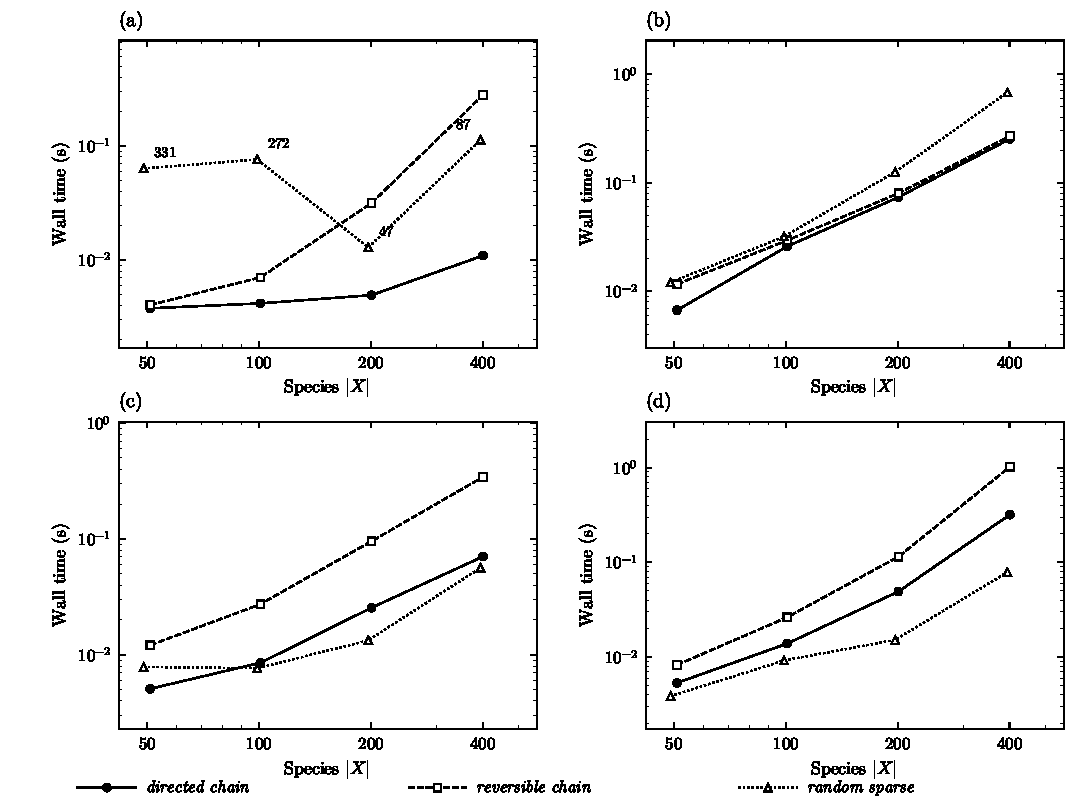
\includegraphics[width=\linewidth]{../Figure/performance_diagnostics.pdf}
    \caption{C++ structural-analysis runtimes across directed-chain, reversible-chain, and random-sparse networks. \textbf{(a)}~Minimal-siphon enumeration. \textbf{(b)}~Exact CRNT analysis. \textbf{(c)}~Graph canonicalization. \textbf{(d)}~Exact conserved-pool enumeration. Points and connecting lines show completed single-run measurements. The key draws a small member of each family (circles: species, bars: bimolecular reactions) beside its line style. All 60 measurements complete.}
    \label{fig:performance_diagnostics}
\end{figure}

\section{BioModels: structural SBML interoperability}
\label{si:biomodels}

The eleven entries in Table~\ref{tab:biomodels_models} benchmark structural \texttt{SBML} exchange across a size-stratified selection from \texttt{BioModels}. Ten models contain reaction structures and pass export and re-import checks without loss of stoichiometric multiplicities, while \texttt{BIOMD0000000562} serves as a reaction-free control.

\begin{table}[htbp]
\centering
\caption{BioModels input inventory and structural results. $m$: species; $r$: directed reactions; $s$: exact rank; $\delta$: deficiency; P: minimal conserved pools; S: minimal siphons; RT: supported structural round trip; Covered: every minimal siphon contains a conserved-pool support. Coverage is the sufficient persistence condition used in the main text, including the vacuous case of no siphons; failure does not prove extinction. Dashes mark analyses inapplicable to the reaction-free control.}
\label{tab:biomodels_models}
\scriptsize
\setlength{\tabcolsep}{3pt}
\begin{tabular}{@{}lrrrrrrcc@{}}
\toprule
Model & $m$ & $r$ & $s$ & $\delta$ & P & S & RT & Covered \\
\midrule
% BEGIN GENERATED: biomodels-models
% Generated from crn-biomodels.json.
\texttt{BIOMD0000000001} & 12 & 17 & 11 & 0 & 1 & 1 & yes & no \\
\texttt{BIOMD0000000010} & 8 & 10 & 5 & 0 & 3 & 3 & yes & yes \\
\texttt{BIOMD0000000051} & 18 & 48 & 18 & 8 & 0 & 0 & yes & yes \\
\texttt{BIOMD0000000064} & 26 & 17 & 17 & 0 & 11 & 8 & yes & no \\
\texttt{BIOMD0000000108} & 9 & 17 & 7 & 8 & 2 & 2 & yes & yes \\
\texttt{BIOMD0000000404} & 29 & 35 & 19 & 13 & 10 & 10 & yes & no \\
\texttt{BIOMD0000000637} & 12 & 35 & 6 & 0 & 6 & 3 & yes & yes \\
\texttt{BIOMD0000000019} & 100 & 125 & 81 & 41 & 19 & 20 & yes & no \\
\texttt{BIOMD0000000175} & 120 & 102 & 94 & 6 & 30 & 26 & yes & no \\
\texttt{BIOMD0000000255} & 504 & 827 & 486 & 317 & 17 & 75 & yes & no \\
\texttt{BIOMD0000000562} & 0 & 0 & -- & -- & -- & -- & -- & -- \\
% END GENERATED: biomodels-models
\bottomrule
\end{tabular}
\end{table}

These benchmarks confirm that \synkit reliably extracts and preserves topological reaction networks and stoichiometric multiplicities across diverse curated models.

\section{KEGG: module structure and glycolysis controls}
\label{si:kegg}
\label{sec:si_case_glycolysis}

The four cached modules in Table~\ref{tab:kegg_modules} are the inputs used in main-text Section~\ref{main:sec:results_kegg}: glycolysis (\texttt{M00001}), pyruvate oxidation (\texttt{M00307}), the citrate cycle (\texttt{M00009}), and the pentose phosphate pathway (\texttt{M00004}). The reported invariants refer to their reduced reaction equations with shared participants retained.

\begin{table}[htbp]
\centering
\caption{Structural results for the four reduced KEGG modules. $m$: species; $r$: directed reactions; $n$: complexes; $\ell$: linkage classes; $s$: rank; $\delta=n-\ell-s$: deficiency; P: minimal conserved pools; S: minimal siphons.}
\label{tab:kegg_modules}
\small
\begin{tabular}{@{}lrrrrrrrr@{}}
\toprule
Module & $m$ & $r$ & $n$ & $\ell$ & $s$ & $\delta$ & P & S \\
\midrule
% BEGIN GENERATED: kegg-modules
% Generated from crn-kegg.json.
\texttt{M00001} & 14 & 15 & 16 & 4 & 11 & 1 & 3 & 3 \\
\texttt{M00307} & 13 & 8 & 14 & 7 & 6 & 1 & 8 & 6 \\
\texttt{M00009} & 22 & 12 & 23 & 11 & 12 & 0 & 12 & 9 \\
\texttt{M00004} & 12 & 12 & 14 & 4 & 10 & 0 & 2 & 4 \\
% END GENERATED: kegg-modules
\bottomrule
\end{tabular}
\end{table}

\subsection{Prescribed glycolytic flux and firing certificate}

The main glycolysis model contains 14 species and 15 directed reactions, with currency metabolites omitted and shared polyphosphate and the ferredoxin bypass retained. The largest minimal conservation support comprises eleven carbohydrate intermediates, with coefficient two on hexoses and one on trioses.

Table~\ref{tab:glycolysis_flux} specifies the requested reaction multiset. Its ten reaction identifiers have a total multiplicity of 15; other reactions have zero requested multiplicity. The initial marking contains one \texttt{alpha-D-Glucose} token and zero tokens of every other species.

\begin{table}[htbp]
\centering
\caption{Non-zero firing counts of the prescribed KEGG glycolysis flux. Identifiers match the cached \texttt{M00001} reaction records.}
\label{tab:glycolysis_flux}
\begin{tabular}{@{}lrlr@{}}
\toprule
Reaction & Count & Reaction & Count \\
\midrule
% BEGIN GENERATED: glycolysis-flux
% Generated from crn-kegg.json.
\texttt{R01786} & 1 & \texttt{R01061} & 2 \\
\texttt{R13199} & 1 & \texttt{R01512} & 2 \\
\texttt{R00756} & 1 & \texttt{R01518} & 2 \\
\texttt{R01068} & 1 & \texttt{R00658} & 2 \\
\texttt{R01015} & 1 & \texttt{R00200} & 2 \\
% END GENERATED: glycolysis-flux
\bottomrule
\end{tabular}
\end{table}

Search explores 30 states and returns the following certificate, with reaction identifiers abbreviated to their numeric suffixes:
\begin{equation}
\begin{split}
(&01786,13199,00756,01068,01015,01061,01061,01512,\\
 &01512,01518,00658,00200,01518,00658,00200).
\end{split}
\end{equation}
Independent verification confirms enabling at every firing, non-negative intermediate markings, and a final marking of two pyruvate tokens, while the weighted carbohydrate pool remains two throughout all 15 steps.

\subsection{Shared-participant and currency controls}

The shared-participant control requests one firing of \texttt{R02189} from one glucose token, comparing the retention of polyphosphate on both reaction sides with cancelling that common incidence. Species order, reaction order, and the net stoichiometric matrix remain identical. Table~\ref{tab:glycolysis_participant} demonstrates that retained polyphosphate must be present for enabling even though its net stoichiometric coefficient is zero.

\begin{table}[htbp]
\centering
\caption{Shared-polyphosphate control for a single prescribed \texttt{R02189} firing. The glucose inventory is one in every row. $n$: complexes; $\ell$: linkage classes; $\delta$: deficiency.}
\label{tab:glycolysis_participant}
\begin{tabular}{@{}lrrrrl@{}}
\toprule
Shared participant & PolyP tokens & $n$ & $\ell$ & $\delta$ & Decision \\
\midrule
% BEGIN GENERATED: glycolysis-participant-control
% Generated from crn-review-experiments.json.
Retained & 0 & 16 & 4 & 1 & blocked \\
Retained & 1 & 16 & 4 & 1 & fires \\
Cancelled & 0 & 14 & 3 & 0 & fires \\
Cancelled & 1 & 14 & 3 & 0 & fires \\
% END GENERATED: glycolysis-participant-control
\bottomrule
\end{tabular}
\end{table}

The currency control applies the 15-firing flux of Table~\ref{tab:glycolysis_flux} to a glucose-only initial marking. Restoring the omitted currency metabolites produces a 24-species model (Table~\ref{tab:glycolysis_currency}). Without ATP supplied, hexokinase cannot fire and exhaustive search confirms that the pathway is unrealizable.

\begin{table}[htbp]
\centering
\caption{Currency-boundary control for the prescribed full glycolytic flux from one glucose and zero tokens of all other species. The negative decision is exhaustive for this reaction multiset.}
\label{tab:glycolysis_currency}
\begin{tabular}{@{}lrrlr@{}}
\toprule
Currency metabolites & Species & Reactions & Decision & Certificate length \\
\midrule
% BEGIN GENERATED: glycolysis-currency-control
% Generated from crn-review-experiments.json.
Removed & 14 & 15 & realizable & 15 \\
Retained & 24 & 15 & unrealizable & -- \\
% END GENERATED: glycolysis-currency-control
\bottomrule
\end{tabular}
\end{table}

\section{Formose: carbon conservation and precursor requirements}
\label{sec:si_case_formose}

Four rules for aldol addition, retro-aldol cleavage, and reversible keto-enol tautomerization iteratively expand formaldehyde and glycolaldehyde seeds. The fourth iteration contains 37 species and 44 reactions, with 54 complexes, 17 linkage classes, rank 36, and deficiency one.

\subsection{Network growth and carbon conservation}

Table~\ref{tab:formose_growth} reports the recorded species and reaction counts across iterations. The fourth iteration includes 31 species containing at least four carbons and reaches ten carbons.

\begin{table}[htbp]
  \centering
  \caption{Network size and cumulative generation time from the seeds through each expansion depth in the original single-run formose study. These timings include first-call overhead; Table~\ref{tab:formose_expansion_comparison} provides the repeated comparison after warm-up.}
  \label{tab:formose_growth}
  \scriptsize
  \setlength{\tabcolsep}{3.5pt}
  \begin{tabular}{rrrr}
  \toprule
  Iteration & Species & Reactions & Cumulative time (s) \\
  \midrule
% BEGIN GENERATED: formose-growth
% Generated from crn-formose.json.
1 & 3 & 1 & 0.029 \\
2 & 5 & 4 & 0.003 \\
3 & 9 & 10 & 0.004 \\
4 & 37 & 44 & 0.010 \\
% END GENERATED: formose-growth
\bottomrule
  \end{tabular}
\end{table}

The stoichiometric matrix $\mathbf S\in\mathbb Z^{37\times44}$ has a one-dimensional left nullspace whose positive primitive conservation vector agrees exactly with the molecular carbon count for every species, confirming that the generated reaction rules strictly conserve carbon.

\subsection{Independent generation checks and expansion runtimes}

The \synkit timings in the cross-tool comparison use the native CRN expander with Lewis hydrogen counts. Table~\ref{tab:formose_hydrogen_comparison} separately compares this implementation with native explicit-hydrogen expansion and the Python/RDKit construction path, so that backend and hydrogen-model differences remain visible.

The same four element-and-bond rules are represented as mapped reaction \texttt{SMARTS} in \synkit and explicit-hydrogen DPO rules in \texttt{M{\O}D}~1.0.0.75 and \texttt{MolFoundry}~0.1.11. The translation preserves mapped atoms and the bonds removed, retained, and added. Both seeds are initially active. Each parallel expansion round requires at least one frontier reactant and excludes mixtures containing two copies of the same species, matching the published \synkit configuration. This mixture policy is a generation setting, not a chemical prohibition. No molecular-size cutoff is imposed. The \synkit task and mixture caps are raised to $2^{60}$, and completed runs are checked for truncation.

Each tool and depth runs in an isolated process pinned to the same logical CPU of an Intel Core Ultra~7 155H, with one warm-up followed by five timed expansions from fresh seeds. Timings include rule and seed parsing, expansion, and construction of each tool's network representation. They exclude imports, engine startup, the fixed \texttt{SMARTS}-to-GML translation, cross-tool identity checks, and structural analyses. \synkit uses its native Lewis-hydrogen expander (RDKit C++~2026.03.1); the other tools use explicit-hydrogen graph rewriting. The measurements therefore compare complete generation interfaces, including their representation and language-interface costs. Python versions, dependency lists, native build fingerprints, all samples, and exported network snapshots are saved with the benchmark evidence.

For each completed run, exported molecular graphs are converted to canonical non-stereochemical SMILES with explicit hydrogens removed. Reactions are compared as directed pairs of reactant and product multisets, preserving multiplicities. The identity check ignores atom maps, rule labels, and alternative atom-level derivations of the same stoichiometric reaction. All three tools return identical species and directed stoichiometric reaction sets at every depth from one through six, including 302 species and 371 reactions at depth five and 10\,572 species and 11\,239 reactions at depth six. Carbon balance is independently checked for every exported reaction. Median times and the first and third quartiles are reported in Table~\ref{tab:formose_expansion_comparison}; Fig.~\ref{fig:formose_expansion_comparison} shows cross-tool runtimes and the implementation controls.

Depth seven does not yield a complete network in the cross-tool comparison under these limits. The \synkit native Lewis worker times out at 180~s during its first expansion; \texttt{M{\O}D} raises \texttt{MemoryError} after approximately 176~s; and \texttt{MolFoundry}'s JavaScript runtime reports an out-of-memory failure and the worker exits with signal~11 after approximately 49~s. Counts and generation-time estimates are therefore withheld for that depth. These resource-limited attempts do not establish an intrinsic maximum expansion depth for any tool.

\begin{table}[htbp]
\centering
\caption{Cumulative formose generation times in seconds: median [first quartile, third quartile] over five runs after one warm-up. Counts describe the completed networks; identity is tested using the complete species and stoichiometric reaction sets. Each worker has a 180~s wall-clock budget covering startup, warm-up, five expansions, and identity audits, and an 8~GiB per-process address-space limit. A timeout or memory failure is an incomplete measurement, not evidence of chemical closure or target unreachability.}
\label{tab:formose_expansion_comparison}
\fontsize{6}{7.2}\selectfont
\setlength{\tabcolsep}{3pt}
\begin{tabular}{rrrlll}
\toprule
Depth & Species & Reactions & \synkit native (Lewis H) & \texttt{M{\O}D} & \texttt{MolFoundry} \\
\midrule
% BEGIN GENERATED: formose-expansion
1 & 3 & 1 & 0.0004862 [0.0004809, 0.0004924] & 0.0003832 [0.000381, 0.0003981] & 0.0121 [0.0112, 0.01235] \\
2 & 5 & 4 & 0.0008686 [0.0008619, 0.0008993] & 0.0005635 [0.0005559, 0.0005639] & 0.02453 [0.01532, 0.03018] \\
3 & 9 & 10 & 0.001607 [0.001603, 0.001689] & 0.000969 [0.0009682, 0.0009777] & 0.02933 [0.01364, 0.03301] \\
4 & 37 & 44 & 0.006683 [0.006673, 0.006729] & 0.002895 [0.002865, 0.002898] & 0.03722 [0.03364, 0.04229] \\
5 & 302 & 371 & 0.07579 [0.07527, 0.07657] & 0.02843 [0.02816, 0.02858] & 0.1745 [0.1684, 0.1745] \\
6 & 10572 & 11239 & 4.293 [4.259, 4.3] & 1.575 [1.566, 1.605] & 11.64 [11.5, 11.7] \\
7 & -- & -- & timeout & memory limit & OOM crash \\
% END GENERATED: formose-expansion
\bottomrule
\end{tabular}
\end{table}

\begin{figure}[htbp]
\centering
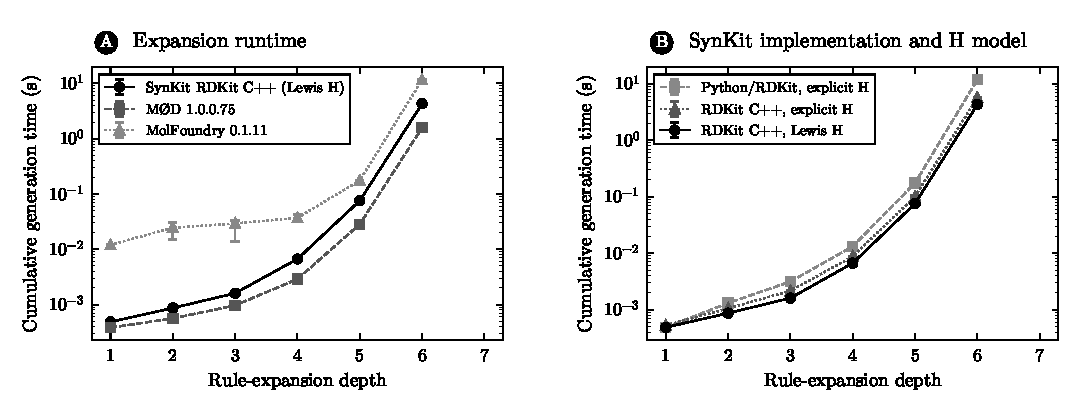
\includegraphics[width=\linewidth]{../Figure/formose_expansion.pdf}
\caption{Formose expansion benchmark. \textbf{(a)}~Median cumulative generation time with first-to-third-quartile error bars over five runs after warm-up. \textbf{(b)}~Controlled comparison of \synkit's Python/RDKit construction path, native explicit-hydrogen expansion, and native Lewis-hydrogen expansion. Lines connect measured depths; incomplete depth-seven runs have no timing point.}
\label{fig:formose_expansion_comparison}
\end{figure}

\begin{table}[htbp]
\centering
\caption{Implementation and hydrogen-representation controls in \synkit~1.6.5. Cumulative generation time in seconds is reported as median [first quartile, third quartile] across five runs after warm-up. The Python control uses \texttt{CRNExpand(rule\_backend="rdkit")}; both native controls use \texttt{rule\_backend="native"}, changing only \texttt{hydrogen\_model}. The Python/RDKit control uses RDKit~2025.09.3, whereas both native controls use RDKit C++~2026.03.1, so the Python--native comparison also includes an RDKit-version difference. The native Lewis column repeats the original comparison measurements. All completed controls reproduce the same complete molecular species and stoichiometric reaction sets. The worker limits match Table~\ref{tab:formose_expansion_comparison}.}
\label{tab:formose_hydrogen_comparison}
\scriptsize
\setlength{\tabcolsep}{3pt}
\begin{tabular}{rlll}
\toprule
Depth & Python/RDKit, explicit H & Native, explicit H & Native, Lewis H \\
\midrule
% BEGIN GENERATED: formose-variants
1 & 0.000488 [0.0004786, 0.0005746] & 0.0005279 [0.0005199, 0.0005556] & 0.0004862 [0.0004809, 0.0004924] \\
2 & 0.001311 [0.001284, 0.001317] & 0.001058 [0.001026, 0.001156] & 0.0008686 [0.0008619, 0.0008993] \\
3 & 0.003154 [0.003039, 0.003355] & 0.002156 [0.002067, 0.002196] & 0.001607 [0.001603, 0.001689] \\
4 & 0.01321 [0.01246, 0.01363] & 0.008774 [0.008767, 0.008798] & 0.006683 [0.006673, 0.006729] \\
5 & 0.1756 [0.173, 0.1761] & 0.1009 [0.1006, 0.1039] & 0.07579 [0.07527, 0.07657] \\
6 & 11.84 [11.75, 11.85] & 5.7 [5.692, 5.747] & 4.293 [4.259, 4.3] \\
7 & memory limit & timeout & timeout \\
% END GENERATED: formose-variants
\bottomrule
\end{tabular}
\end{table}

% BEGIN GENERATED: formose-control-summary
At depth six, median generation times are 11.8~s for Python/RDKit, 5.7~s for native explicit hydrogen, and 4.29~s for native Lewis hydrogen. The native Lewis path is 1.33 times faster than the native explicit-hydrogen path and 2.76 times faster than the Python/RDKit path. A separate instrumented native Lewis control has a median total time of 4.27~s, with 4.09~s in the native request, including transport and decoding, and 0.163~s in Python-side network construction. The native-request measurement combines reaction matching, product sanitization, molecular canonicalization, and protocol costs.
% END GENERATED: formose-control-summary

\subsection{Route definitions and finite precursor inventories}

The targets are an aldotetrose ($T_4$, \texttt{O=CC(O)C(O)CO}) and an aldohexose ($T_6$, \texttt{O=CC(O)C(O)C(O)C(O)CO}). Under qualitative set reachability, both are reachable from the two seed species. Table~\ref{tab:formose_routes} distinguishes qualitative depth from the reaction multiplicities required for discrete firing, and Fig.~\ref{fig:formose_reaction_motifs} shows the reaction motifs.

\begin{table}[htbp]
\centering
\caption{Qualitative depths and prescribed discrete reaction multisets for the selected formose targets. Set reachability reuses a species once generated; discrete firing requires a separate token for each consumed molecule.}
\label{tab:formose_routes}
\begin{tabular}{@{}lrrl@{}}
\toprule
Target & Qualitative depth & Discrete firings & Prescribed multiset \\
\midrule
% BEGIN GENERATED: formose-routes
% Generated from crn-supplement-audit.json.
$T_{4}$ & 2 & 2 & $r_{1}+r_{3}$ \\
$T_{6}$ & 3 & 4 & $2r_{1}+r_{3}+r_{7}$ \\
% END GENERATED: formose-routes
\bottomrule
\end{tabular}
\end{table}

\begin{figure}[!htbp]
\centering
% ---------------------------------------------------------------------------
% formose_chemistry.tex --- the prescribed formose routes as one convergent
% scheme: three glycolaldehyde molecules, two enolizations (r1), the tetrose
% aldol (r3), and the hexose aldol (r7).
%
% Source fragment: loaded by SI/si.tex.
%
% Skeletal structures, hydrogens on carbon implicit.  No atom mapping and no
% stereochemical outcome is asserted: the rule-generated network does not
% assign stereocentres.  Reactions are drawn as Petri-net bars, as in the main
% text, so each glycolaldehyde molecule is a separate input; the shaded block
% is the T4 route (r1 + r3), the whole scheme the T6 route (2 r1 + r3 + r7).
% Black and white, after the shared result-figure style.
% ---------------------------------------------------------------------------
% Figure styles are supplied by the manuscript preamble.

\begingroup
\setchemfig{atom sep=17pt,bond style={line width=0.5pt},bond offset=1.1pt}
\renewcommand*\printatom[1]{\ensuremath{\mathsf{#1}}}
\newcommand{\mfont}{\fontsize{6.5}{7.5}\selectfont\color{black}}
\newcommand{\glycolald}{\chemfig{HO-[:30]-[:-30](-[:30]H)=[:-90]O}}
\newcommand{\enediol}{\chemfig{HO-[:30]=[:-30]-[:30]OH}}
\newcommand{\tetrose}{\chemfig{HO-[:30]-[:-30](-[:-90]OH)-[:30](-[:90]OH)-[:-30](-[:30]H)=[:-90]O}}
\newcommand{\hexose}{\chemfig{HO-[:30]-[:-30](-[:-90]OH)-[:30](-[:90]OH)-[:-30](-[:-90]OH)-[:30](-[:90]OH)-[:-30](-[:30]H)=[:-90]O}}

\begin{tikzpicture}[syn]
\def\W{16.40}
\path[use as bounding box] (0,0) rectangle (\W,-5.25);

\tikzset{
  mol/.style={anchor=center,inner sep=1pt},
  sname/.style={font=\scSmall,text=black,anchor=north,align=center},
  feed/.style={-{Stealth[round,length=1.9mm,width=1.5mm]},line width=0.6pt,
               draw=black},
  rlab/.style={font=\scSmall,text=black,anchor=south,inner sep=1.5pt},
  note/.style={font=\scSmall,text=black,align=left,anchor=north west},
}
% reaction bar: \rbar{name}{x}{y}{label}
\newcommand{\rbar}[4]{%
  \coordinate (#1) at (#2,#3);
  \draw[line width=2.4pt] (#2,#3-0.30) -- (#2,#3+0.30);
  \node[rlab] at (#2,#3+0.30) {#4};
  \coordinate (#1w) at (#2-0.06,#3);
  \coordinate (#1e) at (#2+0.06,#3);}

% Main chain on one line: glycolaldehyde -> r3 -> T4 -> r7 -> T6.  Each aldol
% takes its enediol from a separate enolization, fed from above (r3) or below
% (r7), so the three glycolaldehyde inputs are drawn as three molecules.
\def\ym{-2.35}   % main chain
\def\yt{-0.85}   % first enolization
\def\yl{-4.30}   % second enolization

% --- T4 route (r1 + r3): shaded block --------------------------------------
\fill[black!7] (0.15,-0.12) rectangle (9.85,-3.62);
\node[note] at (0.25,-2.55) {$T_4$ route: $r_1+r_3$\\2 firings\\2 glycolaldehyde};

% --- first enolization (top) and tetrose aldol (main chain) ----------------
\node[mol] (ga) at (1.55,\yt) {\mfont\glycolald};
\rbar{ra}{3.05}{\yt}{$r_1$}
\node[mol] (ea) at (4.40,\yt) {\mfont\enediol};
\draw[feed] (ga.east) -- (raw);
\draw[feed] (rae) -- (ea.west);

\node[mol] (gb) at (4.40,\ym) {\mfont\glycolald};
\rbar{rb}{6.10}{\ym}{$r_3$}
\draw[feed] (ea.east) to[out=0,in=150] (rbw);
\draw[feed] (gb.east) -- (rbw);
\node[mol] (t4) at (8.10,\ym) {\mfont\tetrose};
\draw[feed] (rbe) -- (t4.west);

% --- second enolization (bottom) and hexose aldol (main chain) -------------
\node[mol] (gc) at (5.20,\yl) {\mfont\glycolald};
\rbar{rc}{6.70}{\yl}{$r_1$}
\node[mol] (ec) at (8.10,\yl) {\mfont\enediol};
\draw[feed] (gc.east) -- (rcw);
\draw[feed] (rce) -- (ec.west);

\rbar{rd}{10.55}{\ym}{$r_7$}
\draw[feed] (t4.east) -- (rdw);
\draw[feed] (ec.east) to[out=0,in=-150] (rdw);
\node[mol] (t6) at (13.40,\ym) {\mfont\hexose};
\draw[feed] (rde) -- (t6.west);

% --- names under each structure ---------------------------------------------
\foreach \n/\t in {ga/glycolaldehyde 1, gb/glycolaldehyde 2,
                   gc/glycolaldehyde 3, ea/enediol, ec/enediol}
  \node[sname] at ([yshift=-0.5mm]\n.south) {\t};
\node[sname] at ([yshift=-0.5mm]t4.south) {$T_4$, aldotetrose (C$_4$)};
\node[sname] at ([yshift=-0.5mm]t6.south) {$T_6$, aldohexose (C$_6$)};

\node[note,anchor=north east,align=right] at (16.30,-3.75)
  {$T_6$ route: $2r_1+r_3+r_7$\\4 firings\\3 glycolaldehyde};
\end{tikzpicture}
\endgroup
   % TikZ/chemfig source, typeset inline at \textwidth
\caption{Stoichiometry and precursor requirements of the selected formose routes. \textbf{(a)}~Tautomerization ($r_1$) of glycolaldehyde to enediol. \textbf{(b)}~Aldol coupling ($r_3$) to the aldotetrose ($T_4$). \textbf{(c)}~Second aldol coupling ($r_7$) to the aldohexose ($T_6$). Firing counts are per route. Structures are constitutional; no stereochemistry or atom mapping is assigned.}
\label{fig:formose_reaction_motifs}
\end{figure}

Table~\ref{tab:formose_exact_benchmark} evaluates five initial precursor inventories. Formaldehyde is $C_1$ and glycolaldehyde is $C_2$. Every positive sequence is confirmed by an executable firing sequence, while negative decisions are established by exhaustive search over the prescribed multiset. For an independent check, the same reaction multisets and initial markings are supplied directly to \texttt{MolFoundry}'s \texttt{FlowSolution}, without optimizing a new hyperflow. Its \texttt{is\_realizable()} method and SMT certificate enumeration agree with all ten \synkit decisions. All three positive certificates are independently replayed, checking enabling before every firing, the requested reaction multiplicities, and target production. This comparison concerns the prescribed routes, rather than unrestricted target reachability.

\begin{table}[htbp]
\centering
\caption{Realizability of the prescribed tetrose and hexose routes across five precursor inventories. Counts denote molecules; total carbon counts carbon tokens. Yes indicates a verified certificate and No an exhaustive negative decision for the selected multiset.}
\label{tab:formose_exact_benchmark}
\begin{tabular}{@{}lrrrrr@{}}
\toprule
Pool & $C_1$ count & $C_2$ count & Total carbon & $T_4$ & $T_6$ \\
\midrule
% BEGIN GENERATED: formose-inventories
% Generated from crn-supplement-audit.json.
$M_1$ & 1 & 1 & 3 & no & no \\
$M_2$ & 2 & 1 & 4 & no & no \\
$M_3$ & 4 & 1 & 6 & no & no \\
$M_4$ & 2 & 2 & 6 & yes & no \\
$M_5$ & 0 & 3 & 6 & yes & yes \\
% END GENERATED: formose-inventories
\bottomrule
\end{tabular}
\end{table}

The tetrose route converts glycolaldehyde to enediol ($r_1$), then couples that enediol with a second glycolaldehyde ($r_3$). It requires two glycolaldehyde molecules and leaves formaldehyde untouched; pools $M_4$ and $M_5$ support it, whereas $M_3$ (which contains only one glycolaldehyde) cannot. The hexose route requires two enediol tokens, consuming three glycolaldehyde molecules in total ($2r_1 + r_3 + r_7$), which only pool $M_5$ satisfies. The three six-carbon inventories ($M_3$, $M_4$, and $M_5$) thus produce different realizability outcomes despite having equal total carbon budgets.

\bibliography{../refs}

\end{document}
